\documentclass[14pt]{extarticle}

\usepackage{fontspec}
\setmainfont{Times New Roman}

% размер полей
\usepackage{geometry}
\geometry{a4paper, top=2cm, bottom=2cm, right=1.5cm, left=3cm}

 %debugging
%\usepackage{showframe}

% полуторный интервал
\usepackage{setspace}
\onehalfspacing

% абзацный отступ
\setlength{\parindent}{1.25cm}

% выравнивание текста по ширине
\sloppy

% списки
\usepackage{calc} % арифметические операции с величинами
\usepackage{enumitem}
\setlist{
    nosep,
    leftmargin=0pt,
    itemindent=\parindent + \labelwidth - \labelsep,
}

% подписи к рисункам и таблицам
\usepackage{caption}
\renewcommand{\figurename}{Рисунок}
\renewcommand{\tablename}{Таблица}
\DeclareCaptionFormat{custom}
{
    \textit{#1#2#3}
}
\DeclareCaptionLabelSeparator{custom}{. }
\captionsetup{
    % хз какой это размер - 12 или нет, но выглядит меньше 14
    font=small,
    format=custom,
    labelsep=custom,
}

% картинки
\usepackage{graphicx}

% колонтитулы
\usepackage{fancyhdr}

% картинки и таблицы находятся именно в том месте текста где помещены (атрибут H)
\usepackage{float}

% таблицы
\usepackage{tabularray}

\graphicspath{ {1.2.1/models/} }
\begin{document}
\pagestyle{fancy}
\fancyhead{}
% disable header
\renewcommand{\headrulewidth}{0pt}
\fancyfoot[L]{Дубровских гр 221-361}
\fancyfoot[C]{ЛР 1.2.1}
\fancyfoot[R]{Продажа автотранспорта}
\singlespacing

\newpage
\begin{center}
    Министерство науки и высшего образования Российской Федерации
    Федеральное государственное автономное образовательное учреждение

    высшего образования

    \guillemotleft МОСКОВСКИЙ ПОЛИТЕХНИЧЕСКИЙ УНИВЕРСИТЕТ\guillemotright

    (МОСКОВСКИЙ ПОЛИТЕХ)
\end{center}
\noindent
\bigbreak
\bigbreak
\bigbreak
\bigbreak
\begin{center}
    ЛАБОРАТОРНАЯ РАБОТА 1.2.1

    По курсу Проектирования пользовательских интерфейсов в веб
    \textbf{Определение требований к проектированию интерфейса сайта}
    \bigbreak
    \bigbreak
    \bigbreak
    \bigbreak
    ТЕМА

    \guillemotleft\textbf{САЙТ ДЛЯ ПРОДАЖИ И ПОИСКА АВТОМОБИЛЕЙ}\guillemotright
\end{center}
\noindent
\bigbreak
\bigbreak
\bigbreak
\bigbreak
\bigbreak
\bigbreak
\bigbreak
\bigbreak
\bigbreak
\bigbreak
\hfill Выполнил

\hfill Дубровских Никита Евгеньевич

\hfill Группа 221-361
\bigbreak
\bigbreak
\bigbreak
\hfill Проверил

\hfill Натур ВВ
\vfill
\begin{center}
    Москва, 2024
\end{center}
\newpage
\onehalfspacing


\begin{center}
    \textbf{Лабораторная работа 1.2.1}

    \textbf{ОПРЕДЕЛЕНИЕ ТРЕБОВАНИЙ К ПРОЕКТИРОВАНИЮ ИНТЕРФЕЙСА САЙТА}
\end{center}

\textbf{Цель работы:} сформулировать требования, необходимые для проектирования интерфейса сайта
\bigskip

\textbf{Задачи:}

\begin{enumerate}
    \item Выбрать тематику и продумать дизайн сайта
    \item Провести анализ пяти подобных сайтов (эвристический анализ). Найти достоинства и недостатки интерфейса и функционала. Дать в тексте отчета комментарии по использованию в проектном сайте достоинств аналогов. Для изучения трафика веб-сайтов рекомендован SimilarWeb.com 
    \item Разработать (составить) вопросы к потенциальному заказчику (бриф).
    \item Разработать (составить) вопросы к потенциальным пользователям сайта.
    \item Получить ответы на вопросы брифов.
    \item Проанализировать (дать осмысленные комментарии) полученную информацию.
    \item Сформулировать и записать в отчете требования к разработке интерфейса сайта и мобильного приложения по выбранной тематике. Сформулировать требования: пользовательские, функциональные, бизнес-требования, монетизацию, масштабируемость.
\end{enumerate}
\bigskip

\textbf{Основные термины}

\begin{itemize}
    \item \textit{Бизнес-требования} определяют высокоуровневые цели организации или клиента (потребителя) – заказчика разрабатываемого продукта.
    \item \textit{Пользовательские требования} описывают цели/задачи пользователей системы, которые должны достигаться/выполняться пользователями при помощи создаваемой программной системы. Эти требования часто представляют в виде вариантов использования.
    \item \textit{Функциональные требования} определяют функциональность (поведение) программной системы, которая должна быть создана разработчиками для предоставления возможности выполнения пользователями своих обязанностей в рамках бизнес-требований и в контексте пользовательских требований.
    \item \textit{Масштабируемость} – способность устройства увеличивать свои возможности путем наращивания числа функциональных блоков, выполняющих одни и те же задачи.
    \item \textit{Эвристика} – совокупность приемов и методов, облегчающих решение познавательных, конструктивных, практических задач.
    \item \textit{Монетизация} — это процесс заработка на создаваемом  цифровом контенте. Это могут быть статьи, видеоролики или подкасты.
\end{itemize}
\bigskip

\textbf{Тематика и дизайн сайта}

Тематикой сайта является платформа для размещения объявлений о продаже автомобилей.

Стилем сайта выбран \guillemotleft Flat\guillemotright , так как:
\begin{itemize}
    \item предполагает минимальное использование декоративных элементов и сложных графических эффектов. Это делает интерфейс более чистым и понятным, что особенно важно для пользователей, которые ищут информацию о машинах. Простота в дизайне способствует лучшему восприятию контента и облегчает навигацию;
    \item акцентирует внимание на контенте, делая его более доступным. Четкие шрифты, яркие кнопки и контрастные цвета позволяют пользователям быстро находить нужные объявления, что критично для сайтов с большим количеством информации;
    \item хорошо подходит для адаптивных веб-сайтов. Он обеспечивает эффективное отображение на различных устройствах — от мобильных телефонов до десктопов. В условиях роста мобильного трафика важно, чтобы сайт был удобен для пользователей на любом устройстве;
    \item не требует использования тяжелых графических элементов и сложных эффектов, это может значительно снизить время загрузки страниц. Быстрая загрузка улучшает пользовательский опыт и влияет на SEO-оптимизацию;
    \item ассоциируется с современными тенденциями веб-дизайна и может помочь создать у пользователей ощущение, что сайт является актуальным и надежным. Это особенно важно для торговых платформ, где доверие играет ключевую роль;
    \item благодаря простоте структуры flat-дизайна, изменения и обновления на сайте можно вносить быстрее и легче. Это важно для платформ с динамическим контентом, таких как сайты объявлений;
    \item позволяет сосредоточиться на функциональности сайта, что помогает пользователям легко выполнять такие действия, как поиск, фильтрация и сортировка объявлений, без отвлечения на ненужные визуальные элементы.
\end{itemize}

Типом сайта является доска объявлений, так как она позволяет пользователям легко размещать, просматривать и фильтровать объявления о продаже автомобилей, создавая удобную и эффективную платформу для взаимодействия между покупателями и продавцами.
\bigskip

\textbf{Анализ подобных сайтов. Определение достоинств и недостатков.}

Для того чтобы выявить лучшие практики, понять потребности целевой аудитории и определить конкурентные преимущества, был проведен анализ сайтов конкурентов. Из наиболее популярных выделены:

\begin{itemize}
    \item auto.ru;
    \item drom.ru;
    \item sberauto.com;
    \item mobile.de;
    \item autoscout24.com.
\end{itemize}

Ниже представлен дизайн сайтов конкурентов в виде скриншотов.
\bigskip

Скриншоты сайта-конкурента \textbf{auto.ru}.

\noindent
\begin{minipage}{\linewidth}
    \fbox{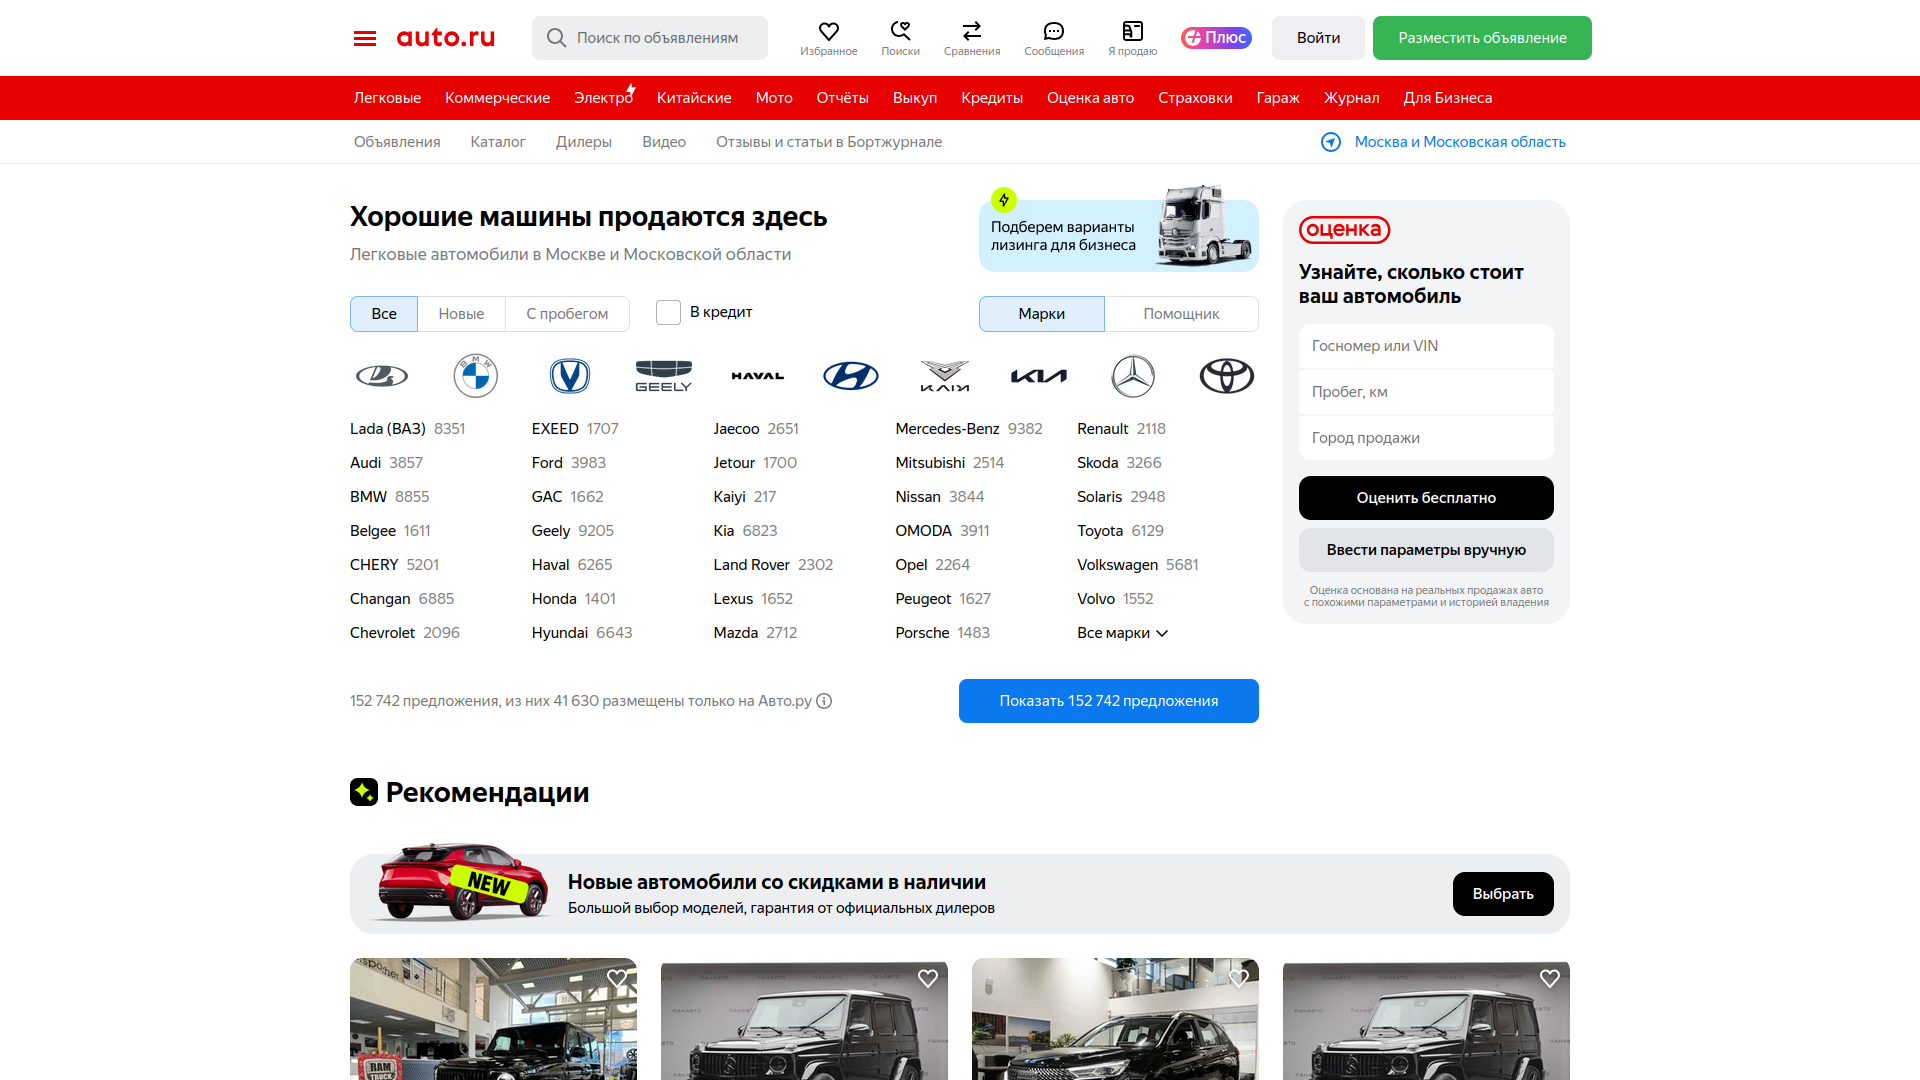
\includegraphics[width=\linewidth]{auto.ru}}
    \captionof{figure}{Скриншот главной страницы сайта auto.ru}
\end{minipage}
\bigskip

\noindent
\begin{minipage}{\linewidth}
    \fbox{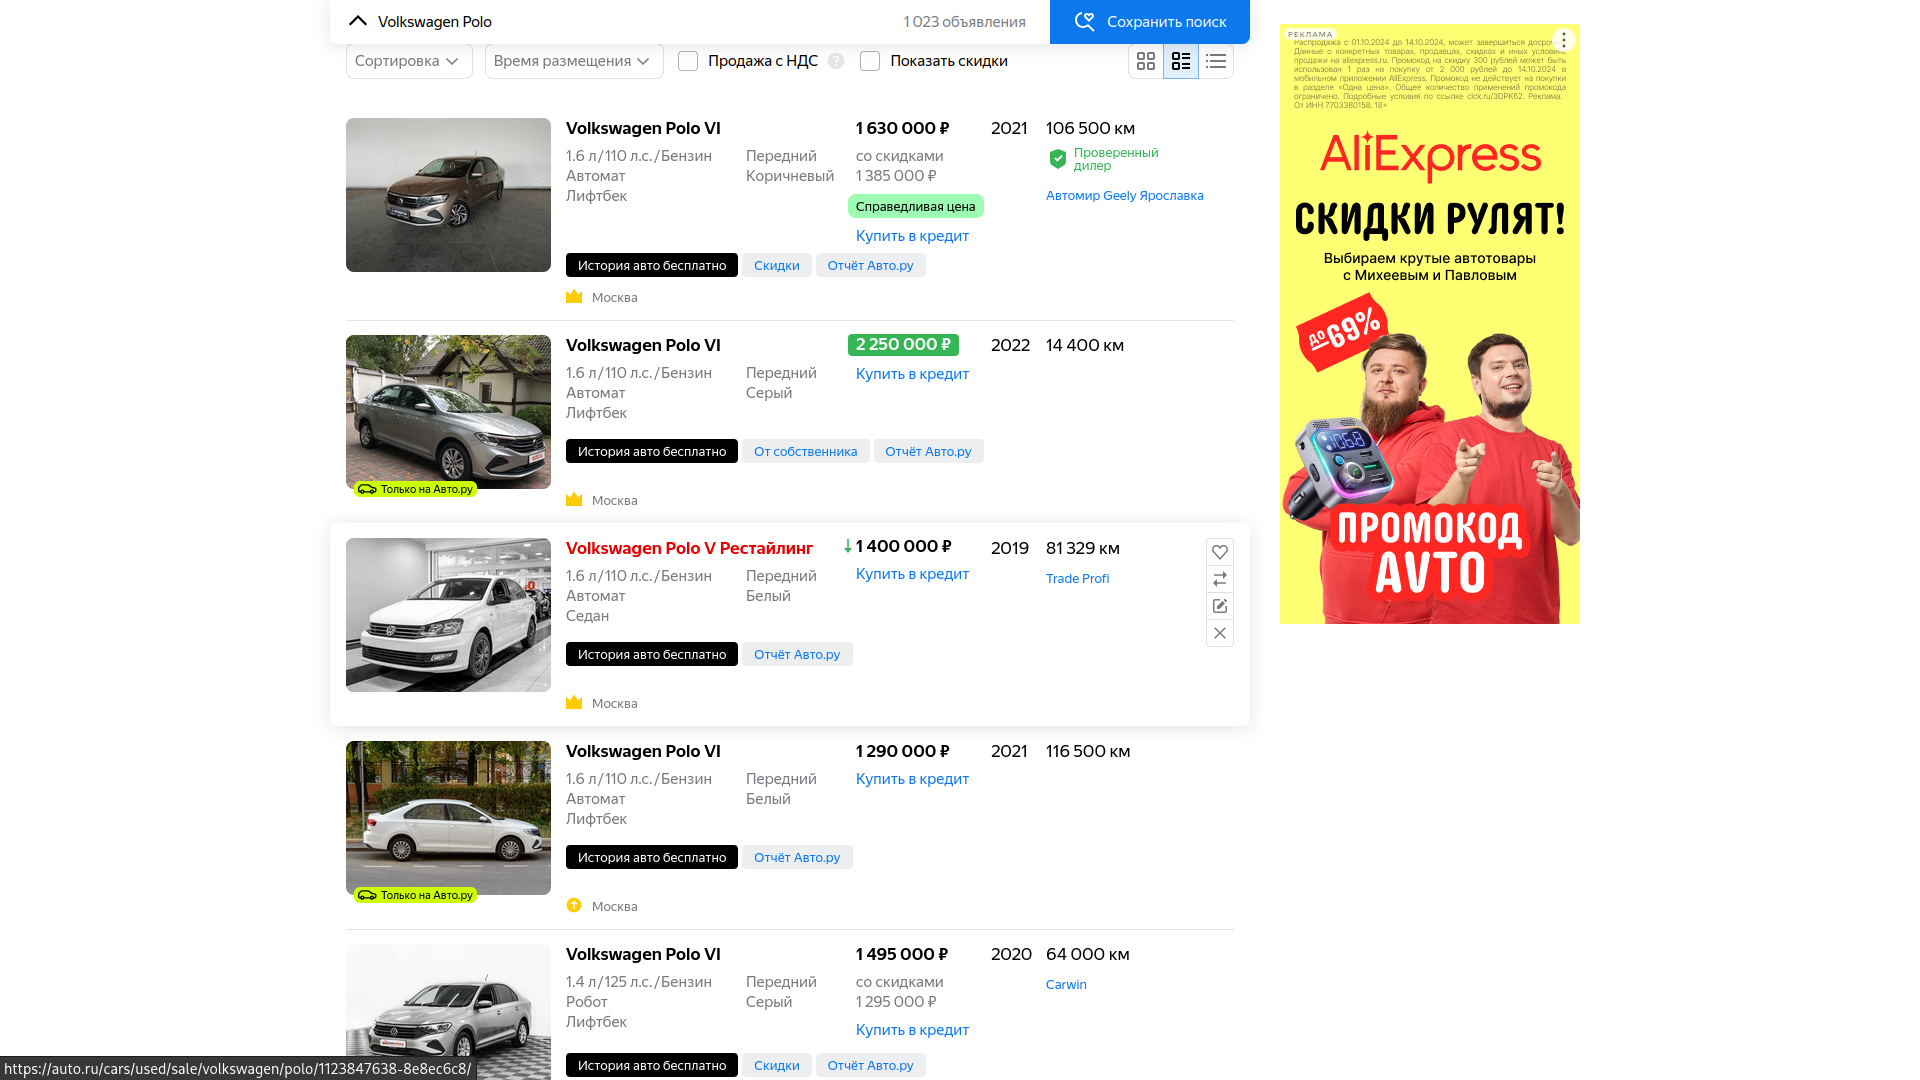
\includegraphics[width=\linewidth]{auto.ru2}}
    \captionof{figure}{Скриншот каталога автомобилей сайта auto.ru}
\end{minipage}
\bigskip

\noindent
\begin{minipage}{\linewidth}
    \fbox{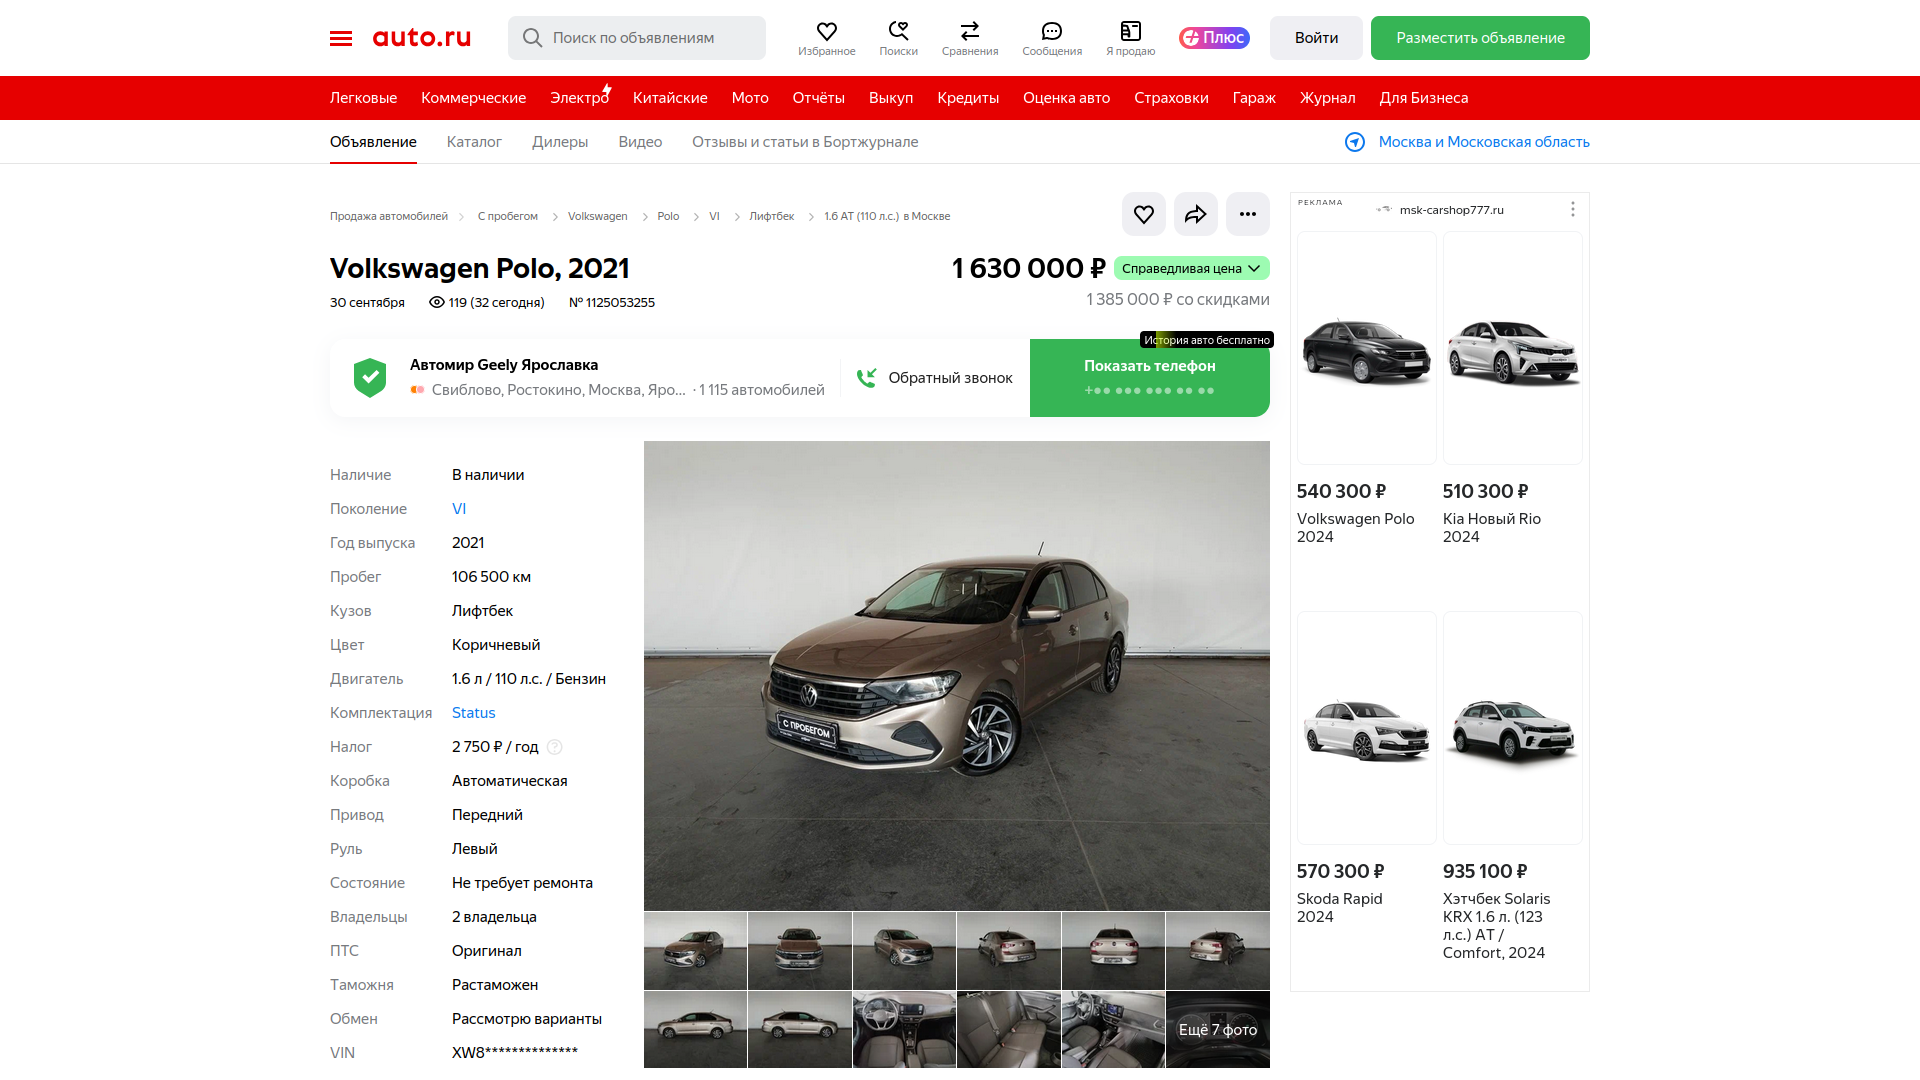
\includegraphics[width=\linewidth]{auto.ru3}}
    \captionof{figure}{Скриншот страницы выбора конкретного автомобиля сайта auto.ru}
\end{minipage}
\bigskip

Скриншоты сайта-конкурента \textbf{drom.ru}.

\noindent
\begin{minipage}{\linewidth}
    \fbox{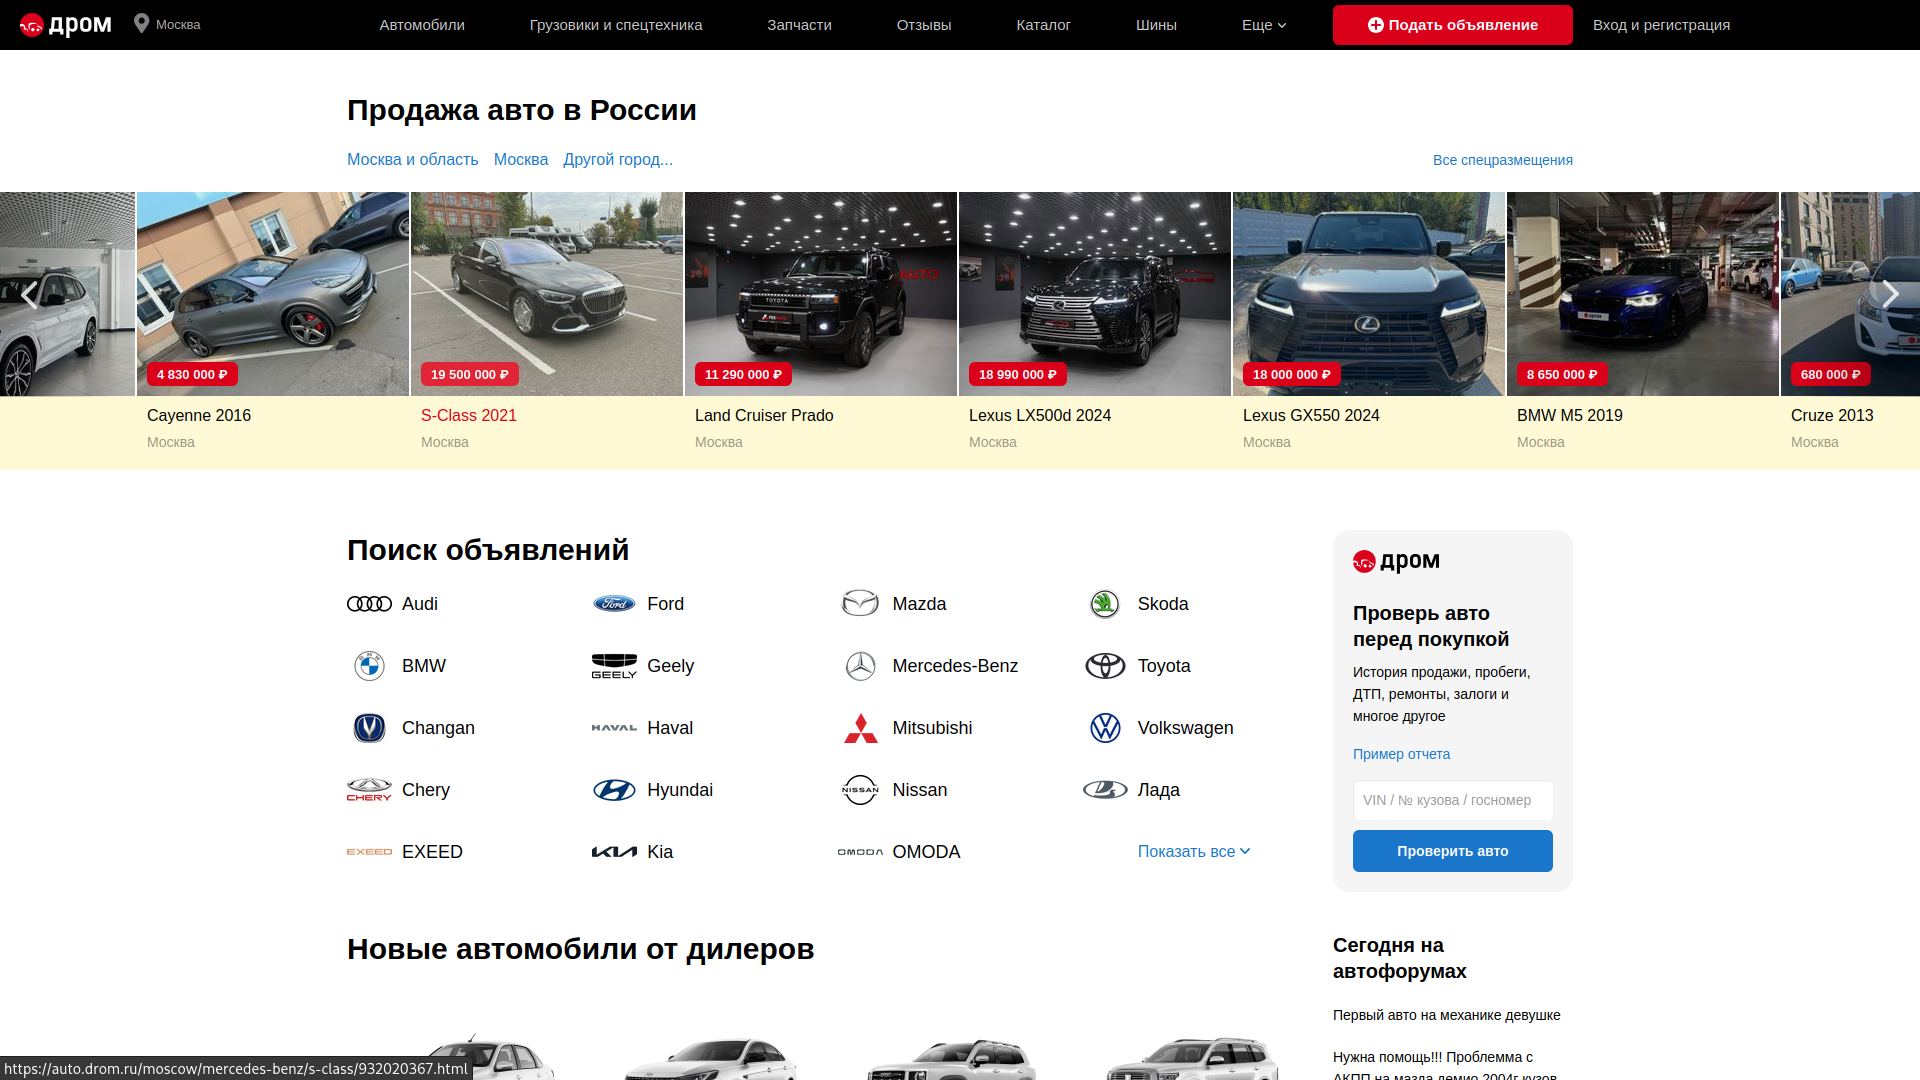
\includegraphics[width=\linewidth]{drom.ru}}
    \captionof{figure}{Скриншот главной страницы сайта drom.ru}
\end{minipage}
\bigskip

\noindent
\begin{minipage}{\linewidth}
    \fbox{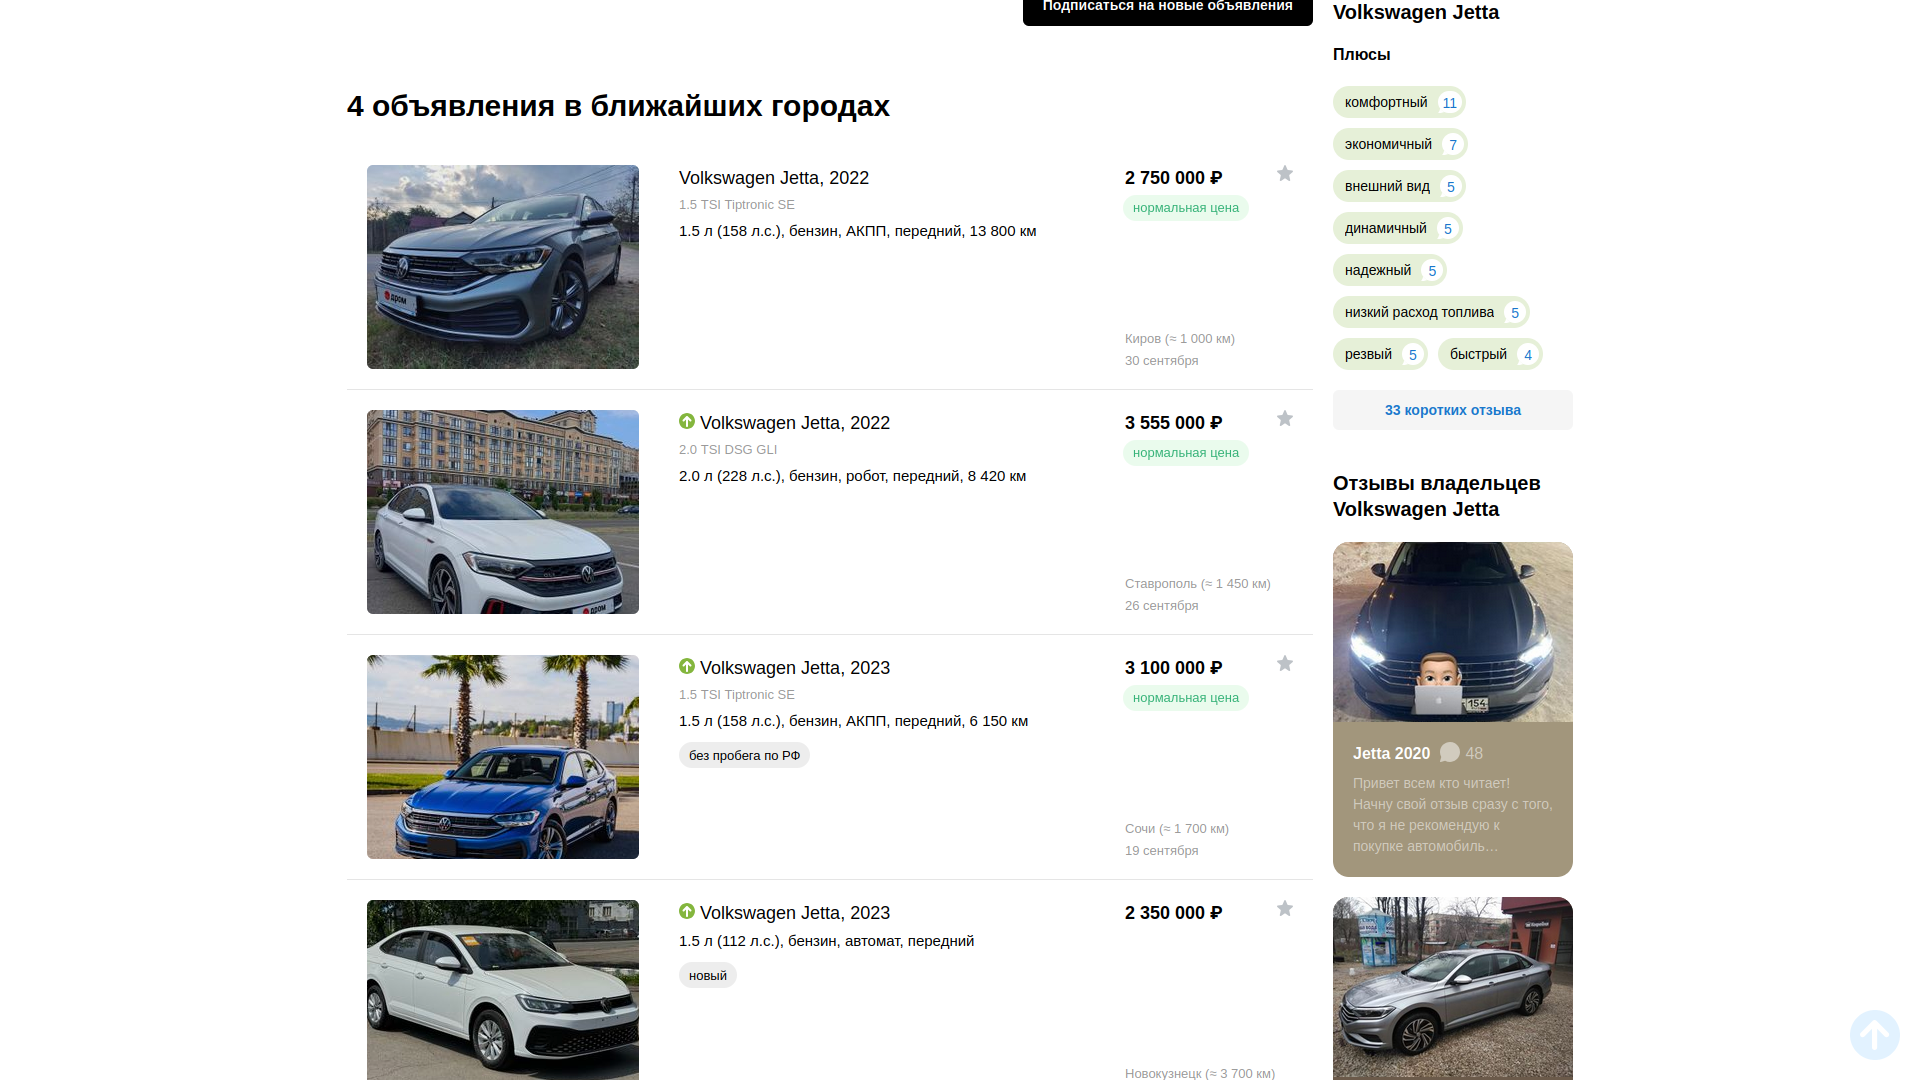
\includegraphics[width=\linewidth]{drom.ru2}}
    \captionof{figure}{Скриншот каталога автомобилей сайта drom.ru}
\end{minipage}
\bigskip

\noindent
\begin{minipage}{\linewidth}
    \fbox{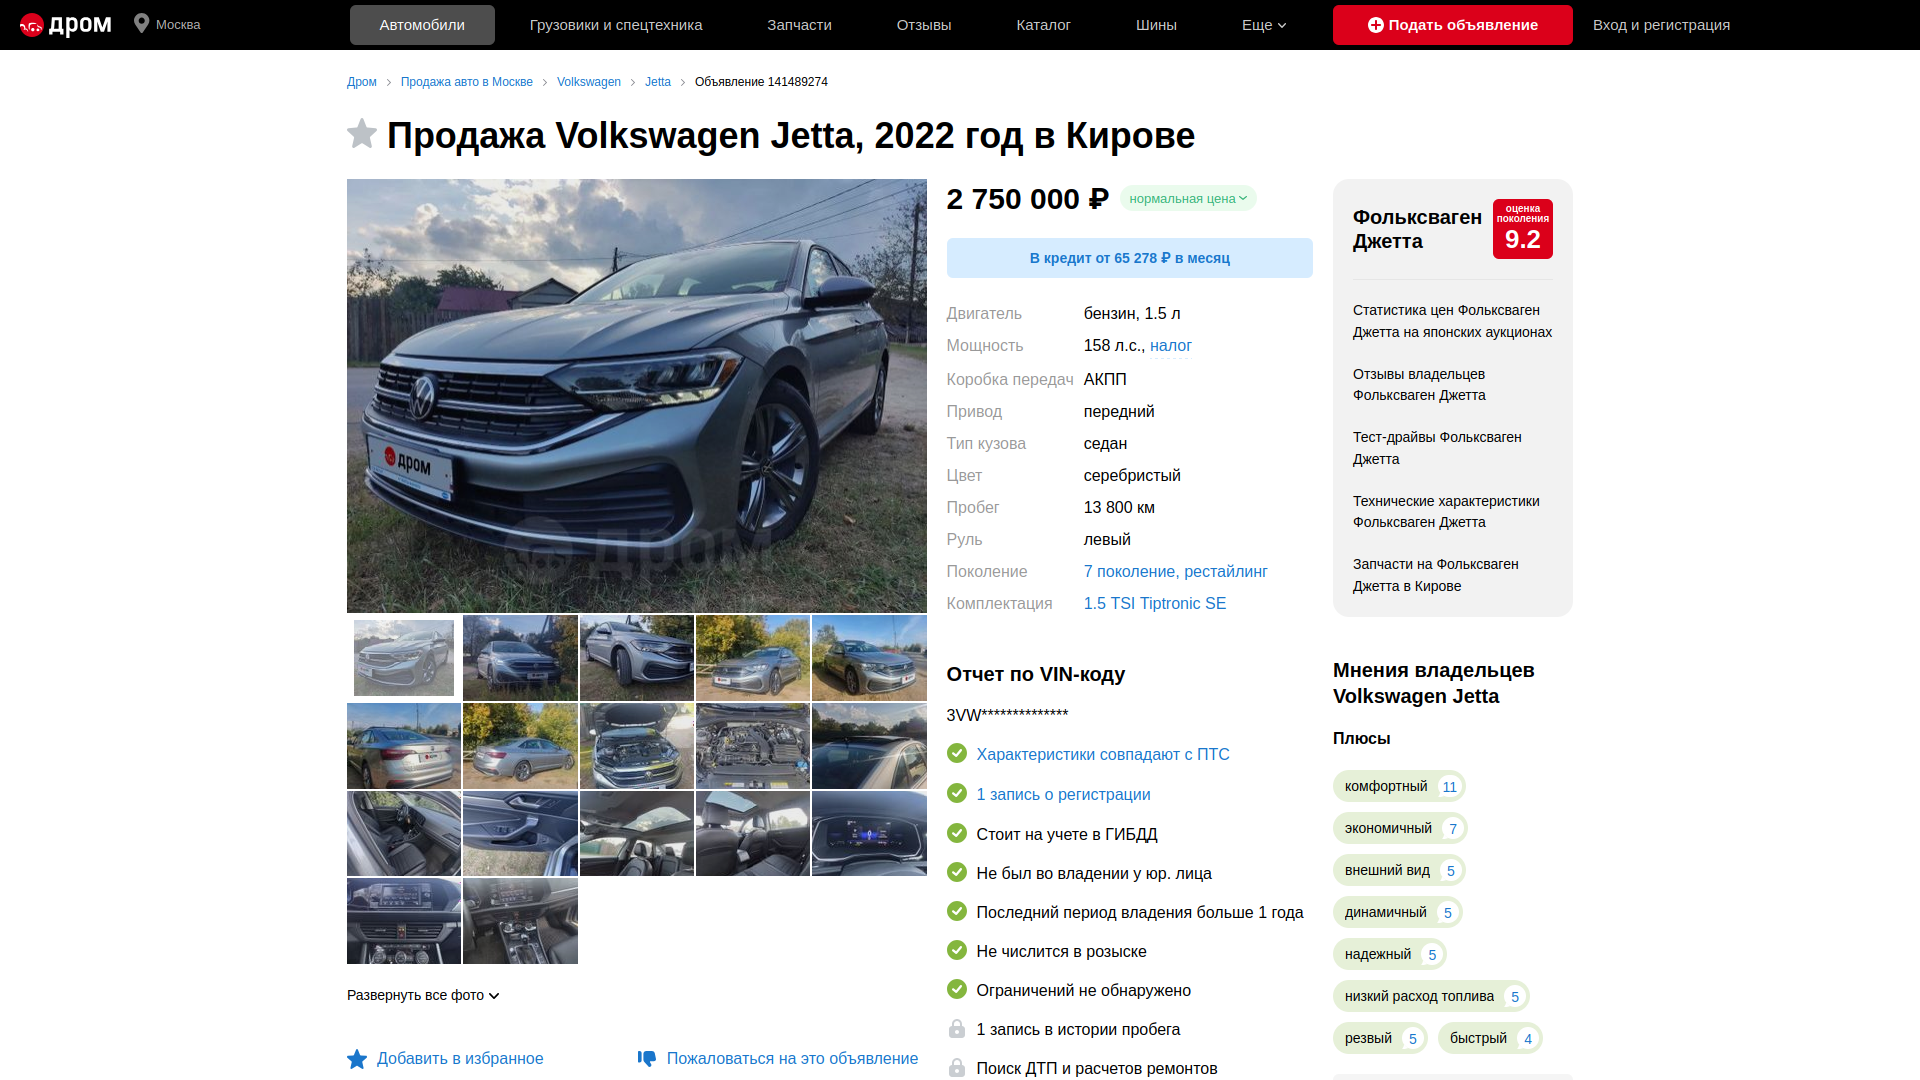
\includegraphics[width=\linewidth]{drom.ru3}}
    \captionof{figure}{Скриншот страницы выбора конкретного автомобиля сайта drom.ru}
\end{minipage}
\bigskip

Скриншоты сайта-конкурента \textbf{sberauto.com}.

\noindent
\begin{minipage}{\linewidth}
    \fbox{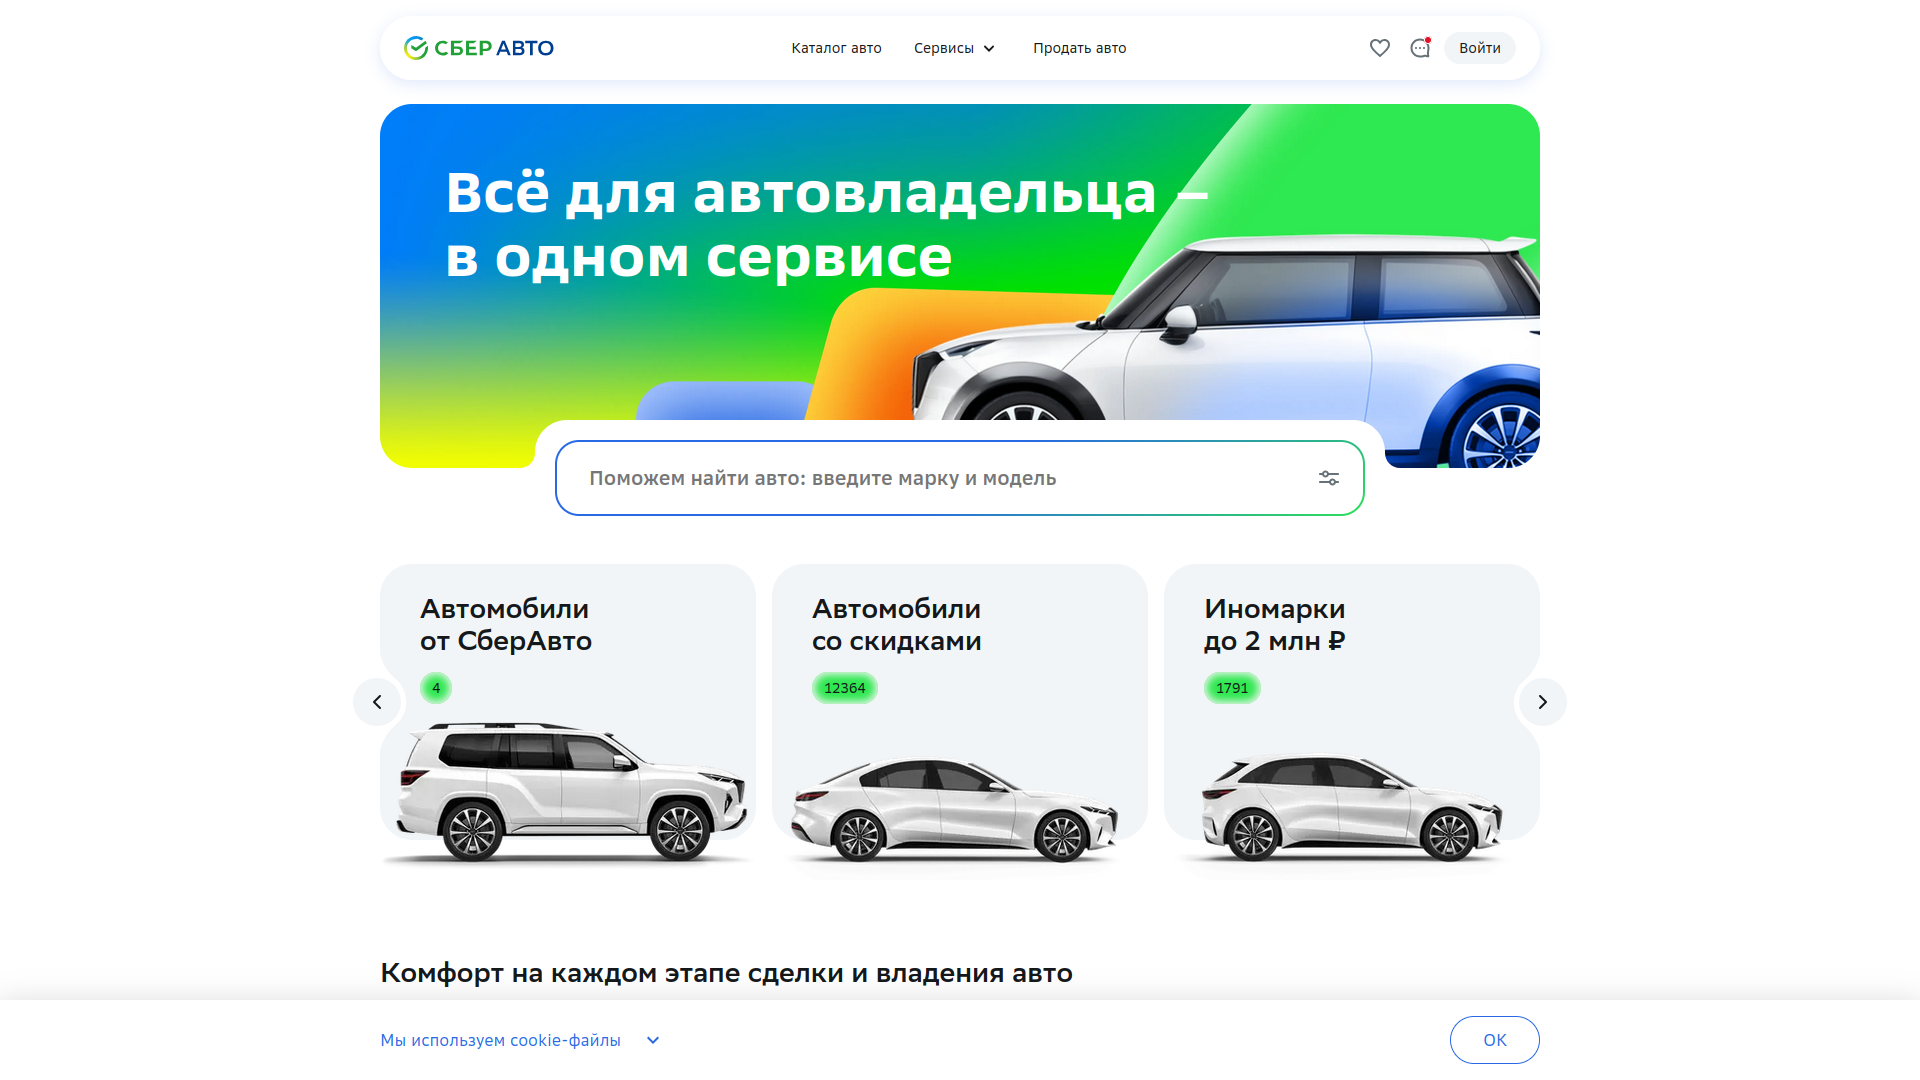
\includegraphics[width=\linewidth]{sberauto.com}}
    \captionof{figure}{Скриншот главной страницы сайта sberauto.com}
\end{minipage}
\bigskip

\noindent
\begin{minipage}{\linewidth}
    \fbox{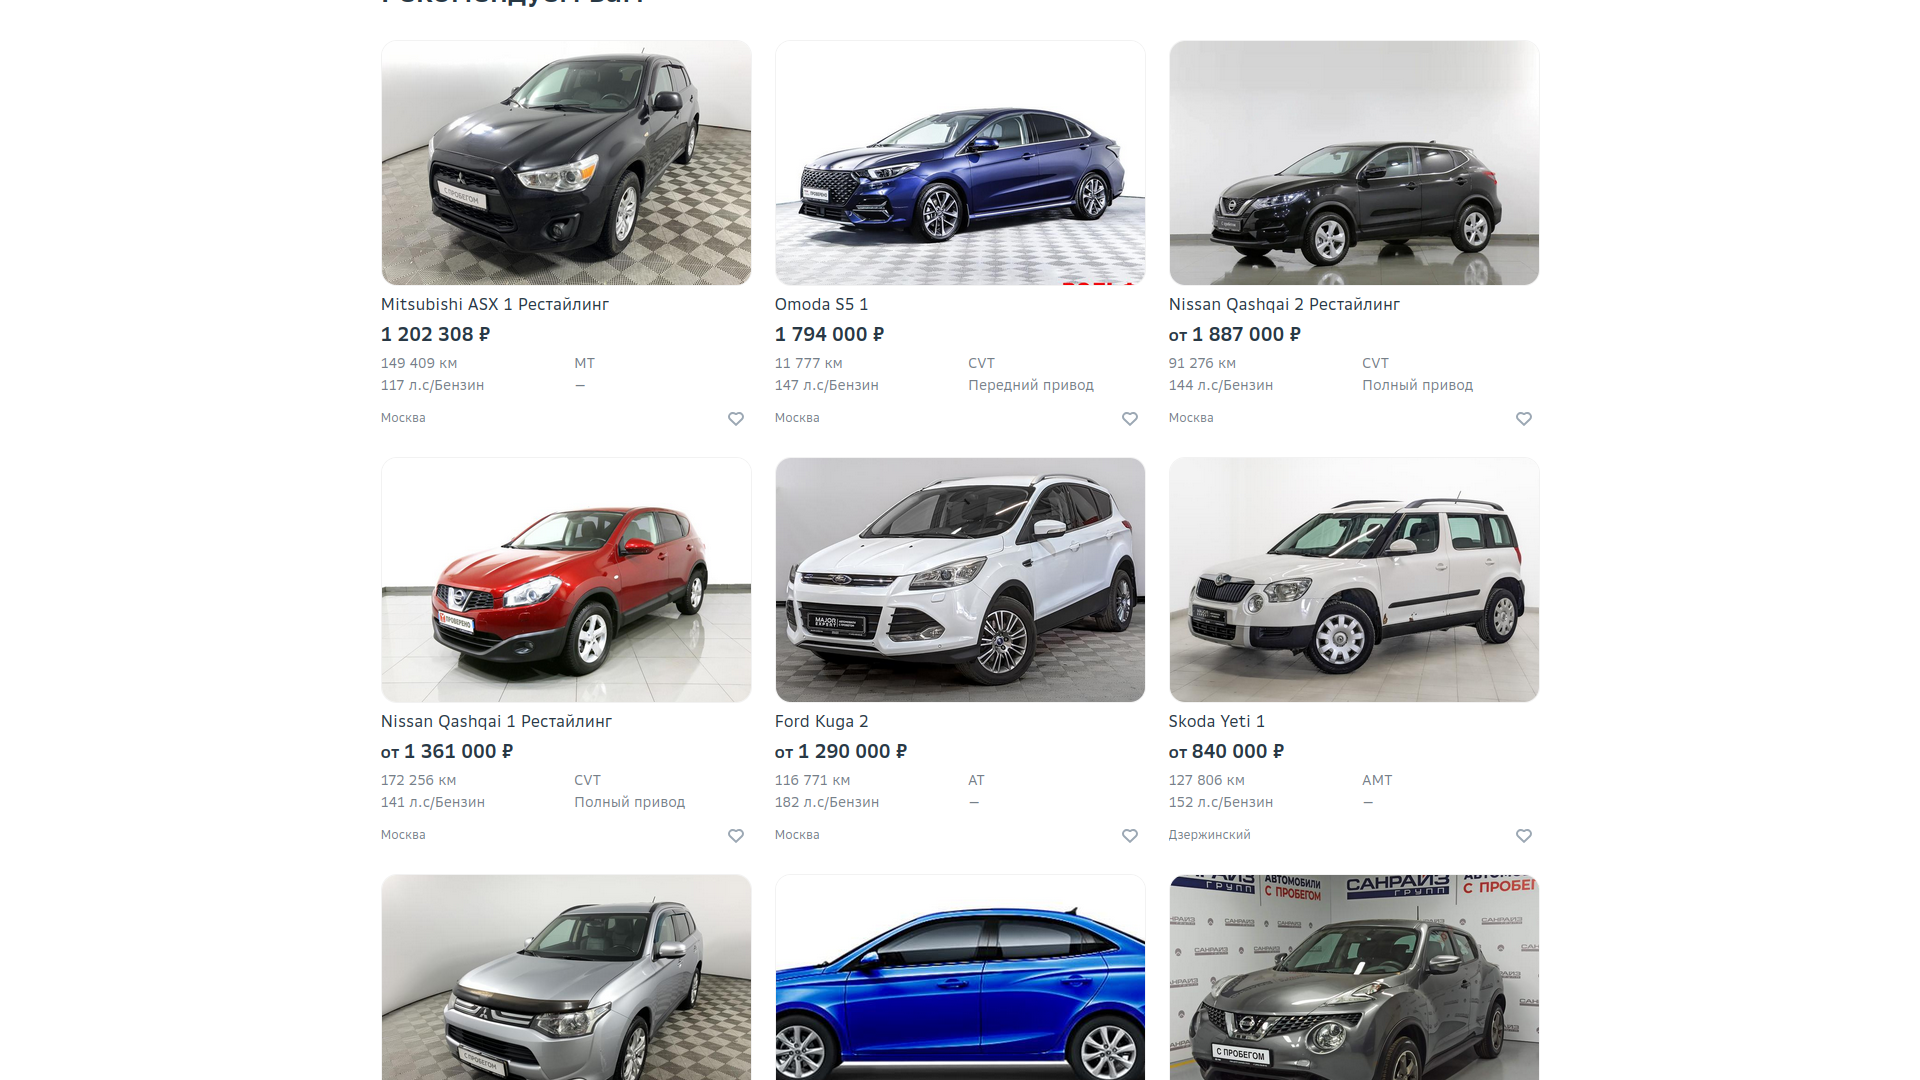
\includegraphics[width=\linewidth]{sberauto.com2}}
    \captionof{figure}{Скриншот каталога автомобилей сайта sberauto.com}
\end{minipage}
\bigskip

\noindent
\begin{minipage}{\linewidth}
    \fbox{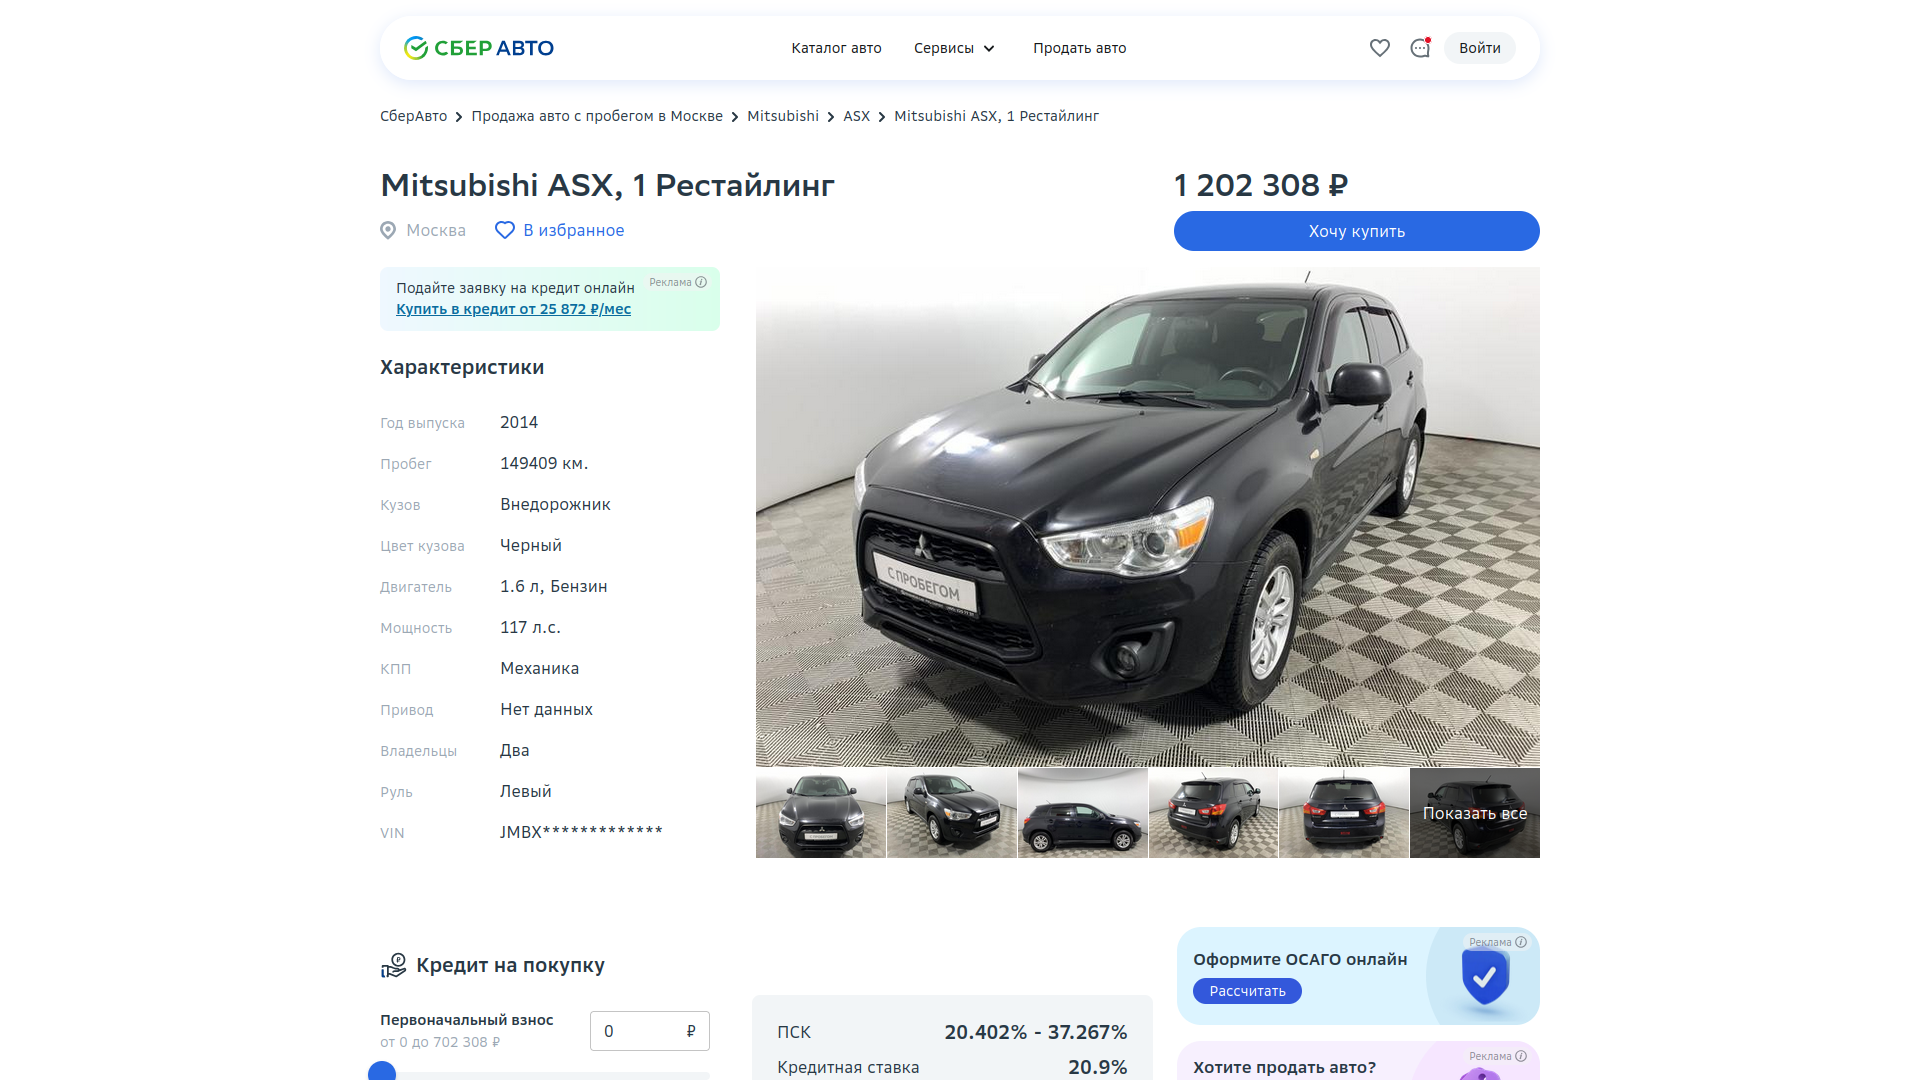
\includegraphics[width=\linewidth]{sberauto.com3}}
    \captionof{figure}{Скриншот страницы выбора конкретного автомобиля сайта sberauto.com}
\end{minipage}
\bigskip

Скриншоты сайта-конкурента \textbf{mobile.de}.

\noindent
\begin{minipage}{\linewidth}
    \fbox{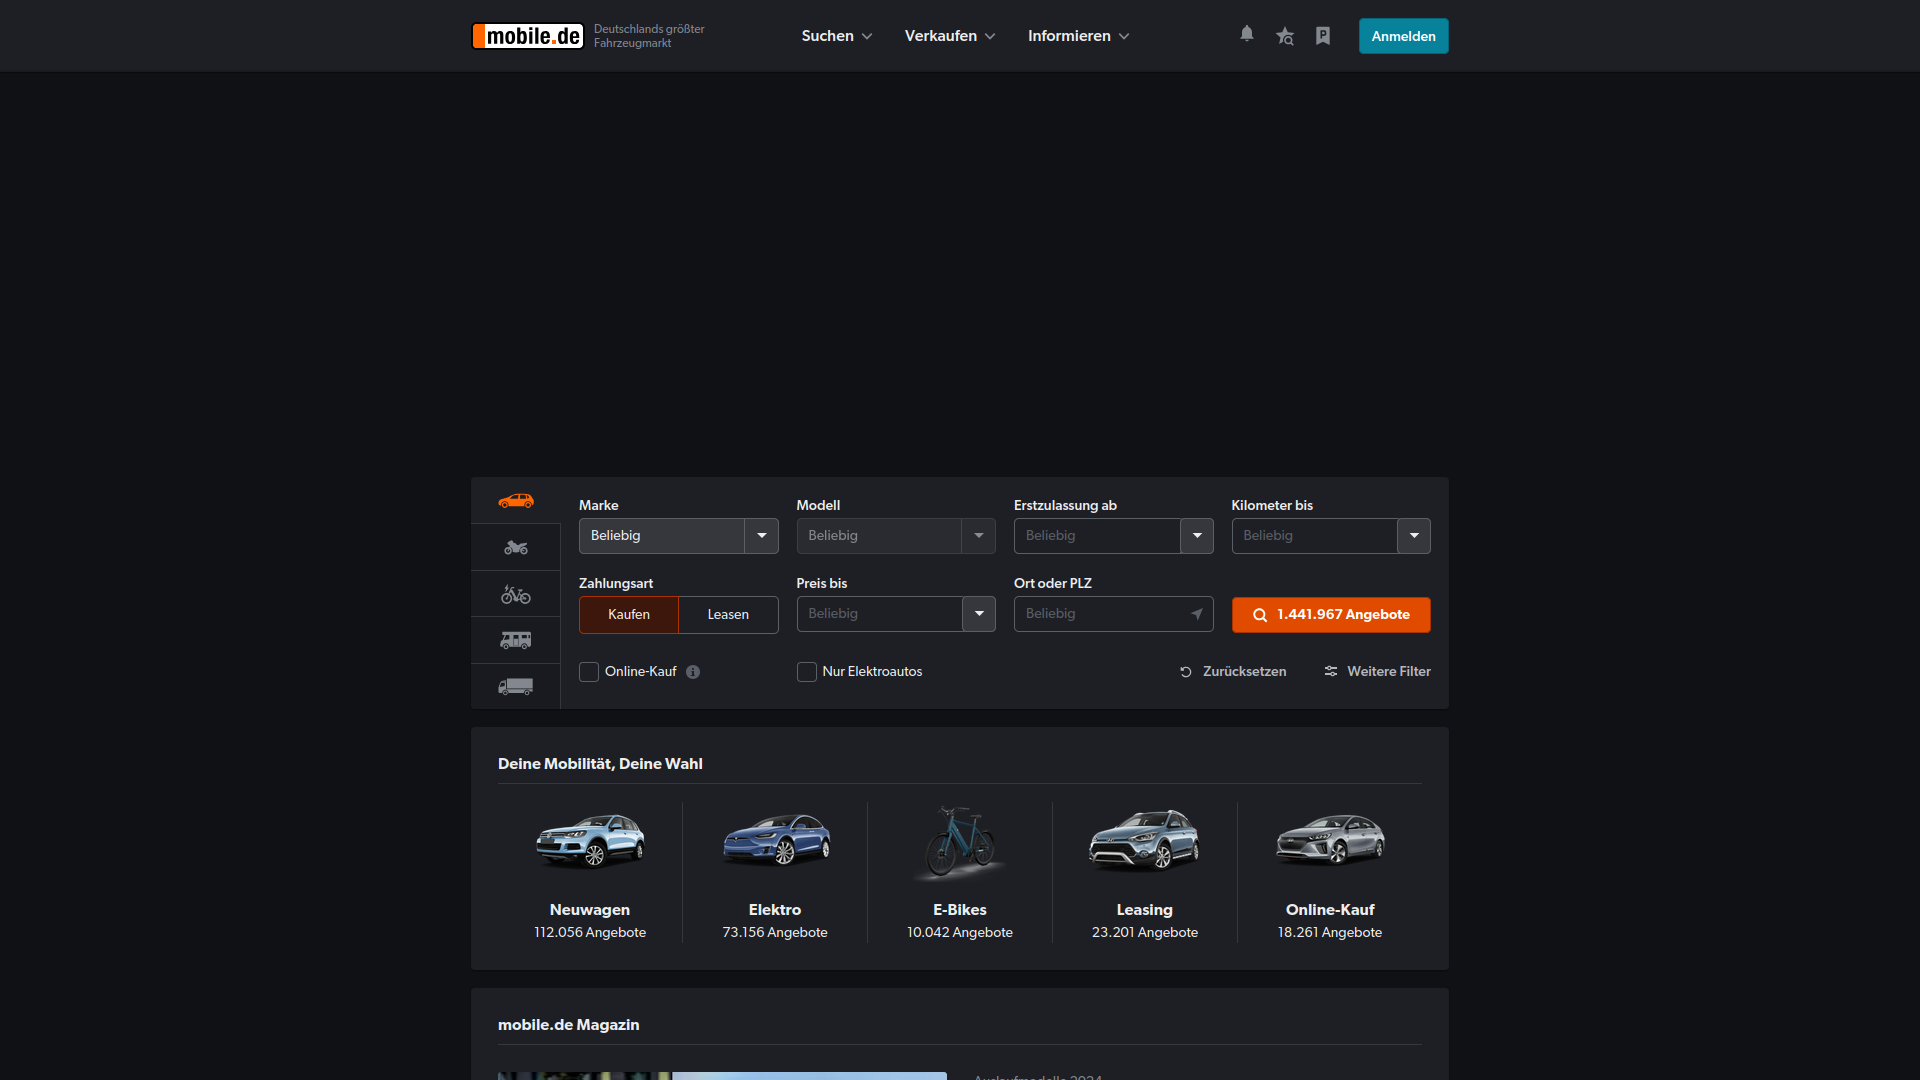
\includegraphics[width=\linewidth]{mobile.de}}
    \captionof{figure}{Скриншот главной страницы сайта mobile.de}
\end{minipage}
\bigskip

\noindent
\begin{minipage}{\linewidth}
    \fbox{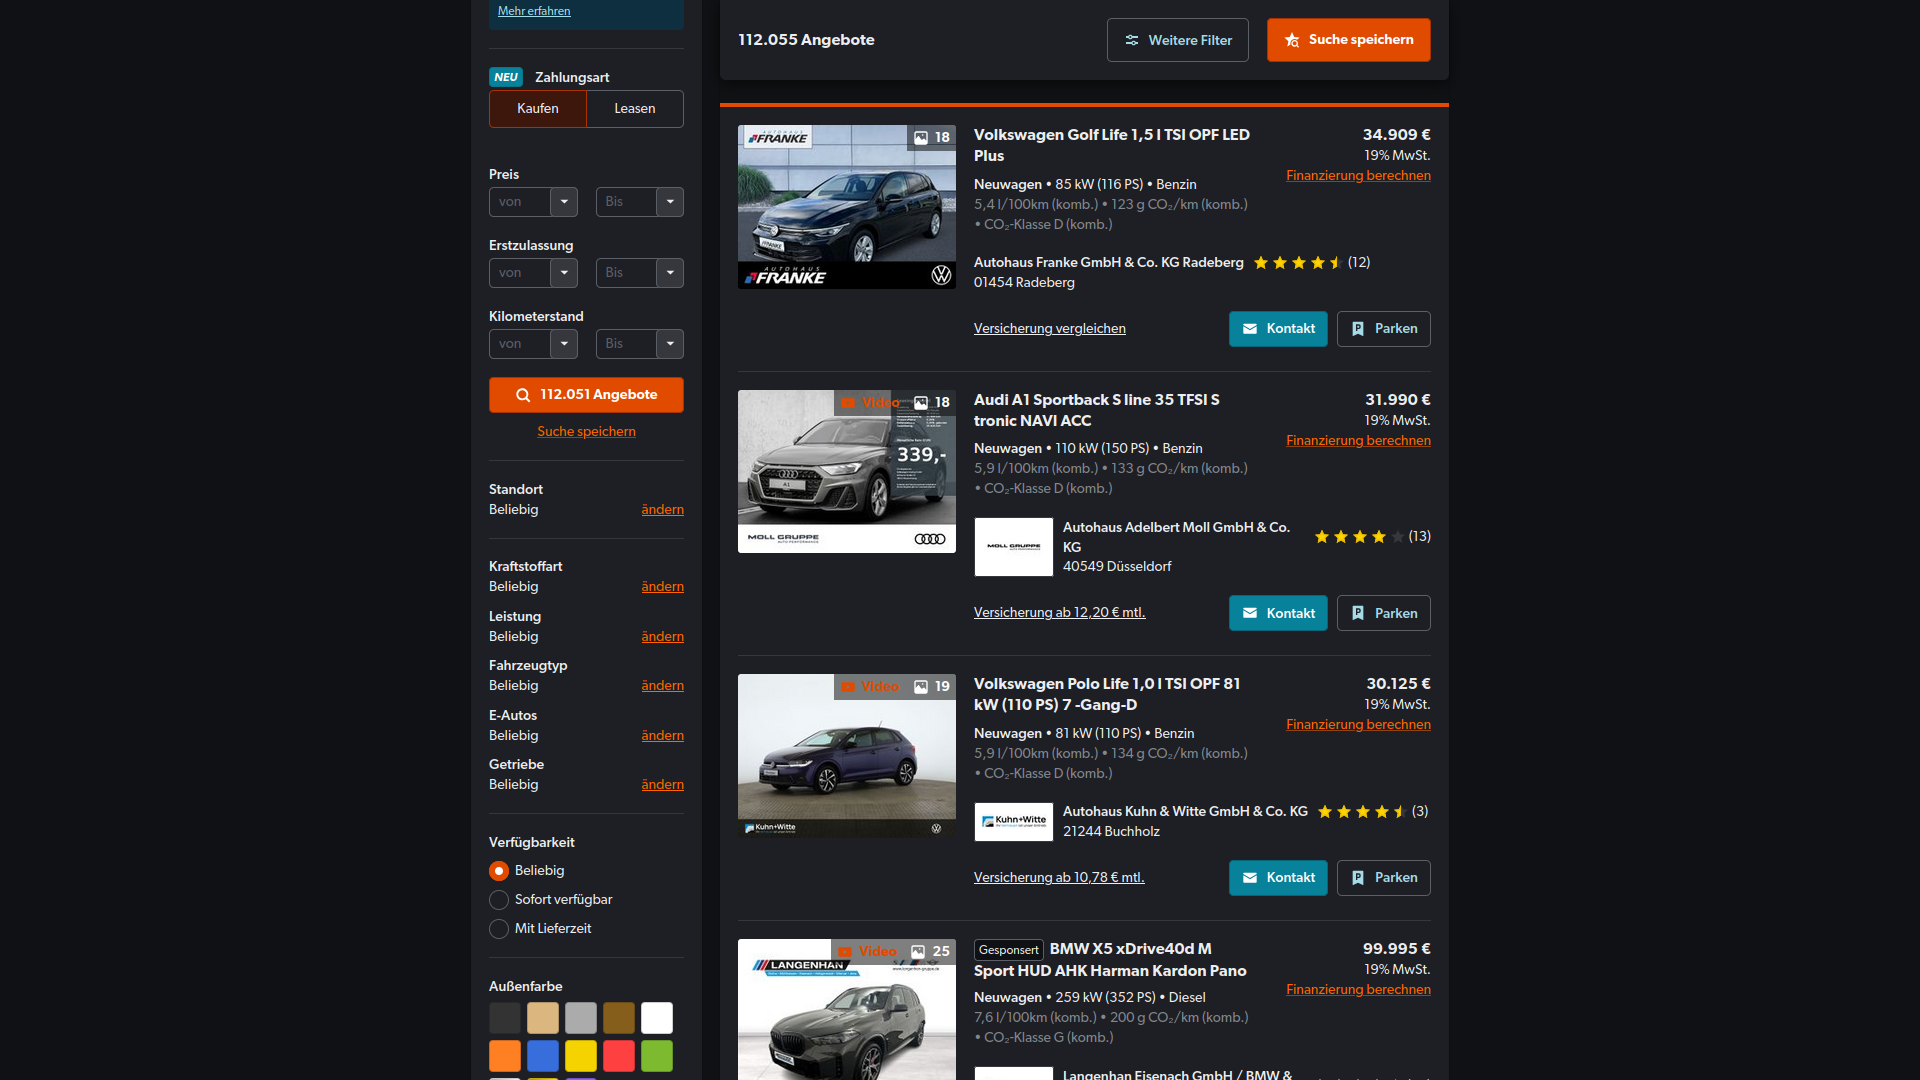
\includegraphics[width=\linewidth]{mobile.de2}}
    \captionof{figure}{Скриншот каталога автомобилей сайта mobile.de}
\end{minipage}
\bigskip

\noindent
\begin{minipage}{\linewidth}
    \fbox{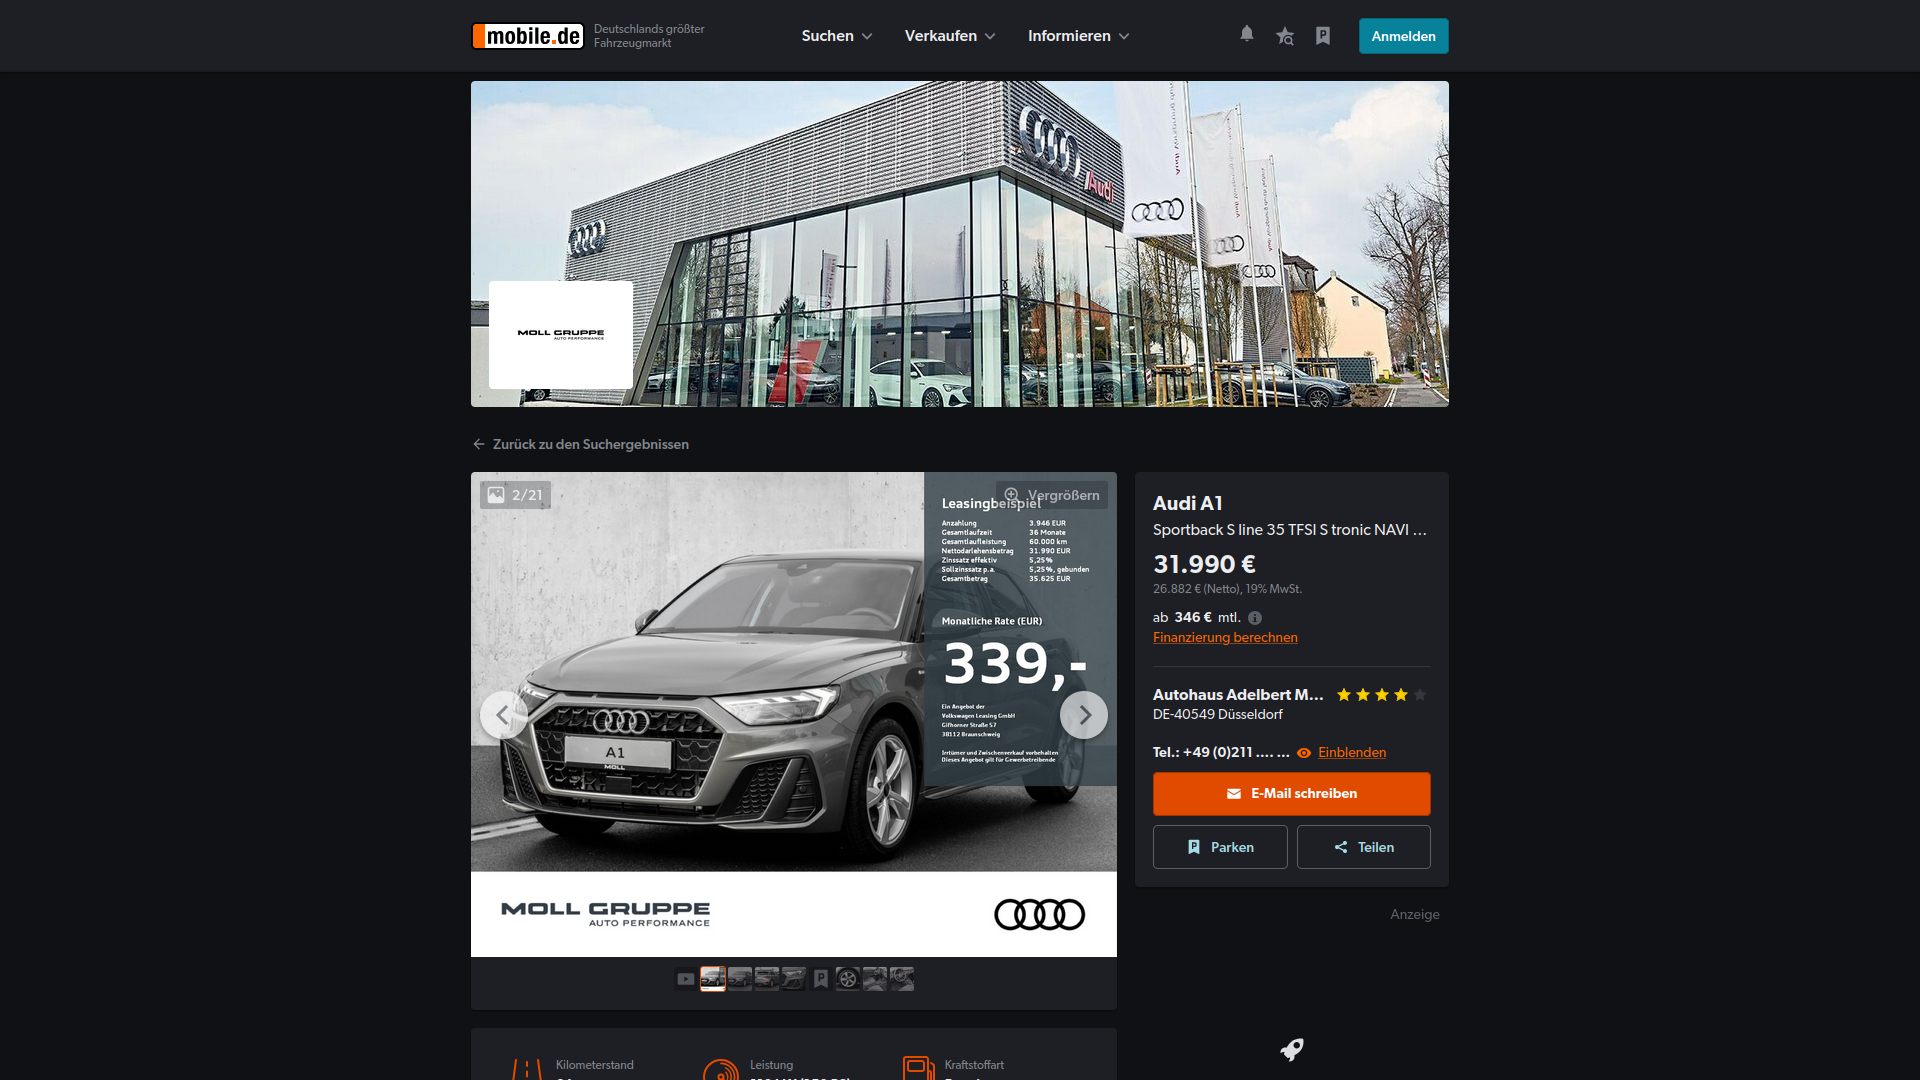
\includegraphics[width=\linewidth]{mobile.de3}}
    \captionof{figure}{Скриншот страницы выбора конкретного автомобиля сайта mobile.de}
\end{minipage}
\bigskip

Скриншоты сайта-конкурента \textbf{autoscout24.com}.

\noindent
\begin{minipage}{\linewidth}
    \fbox{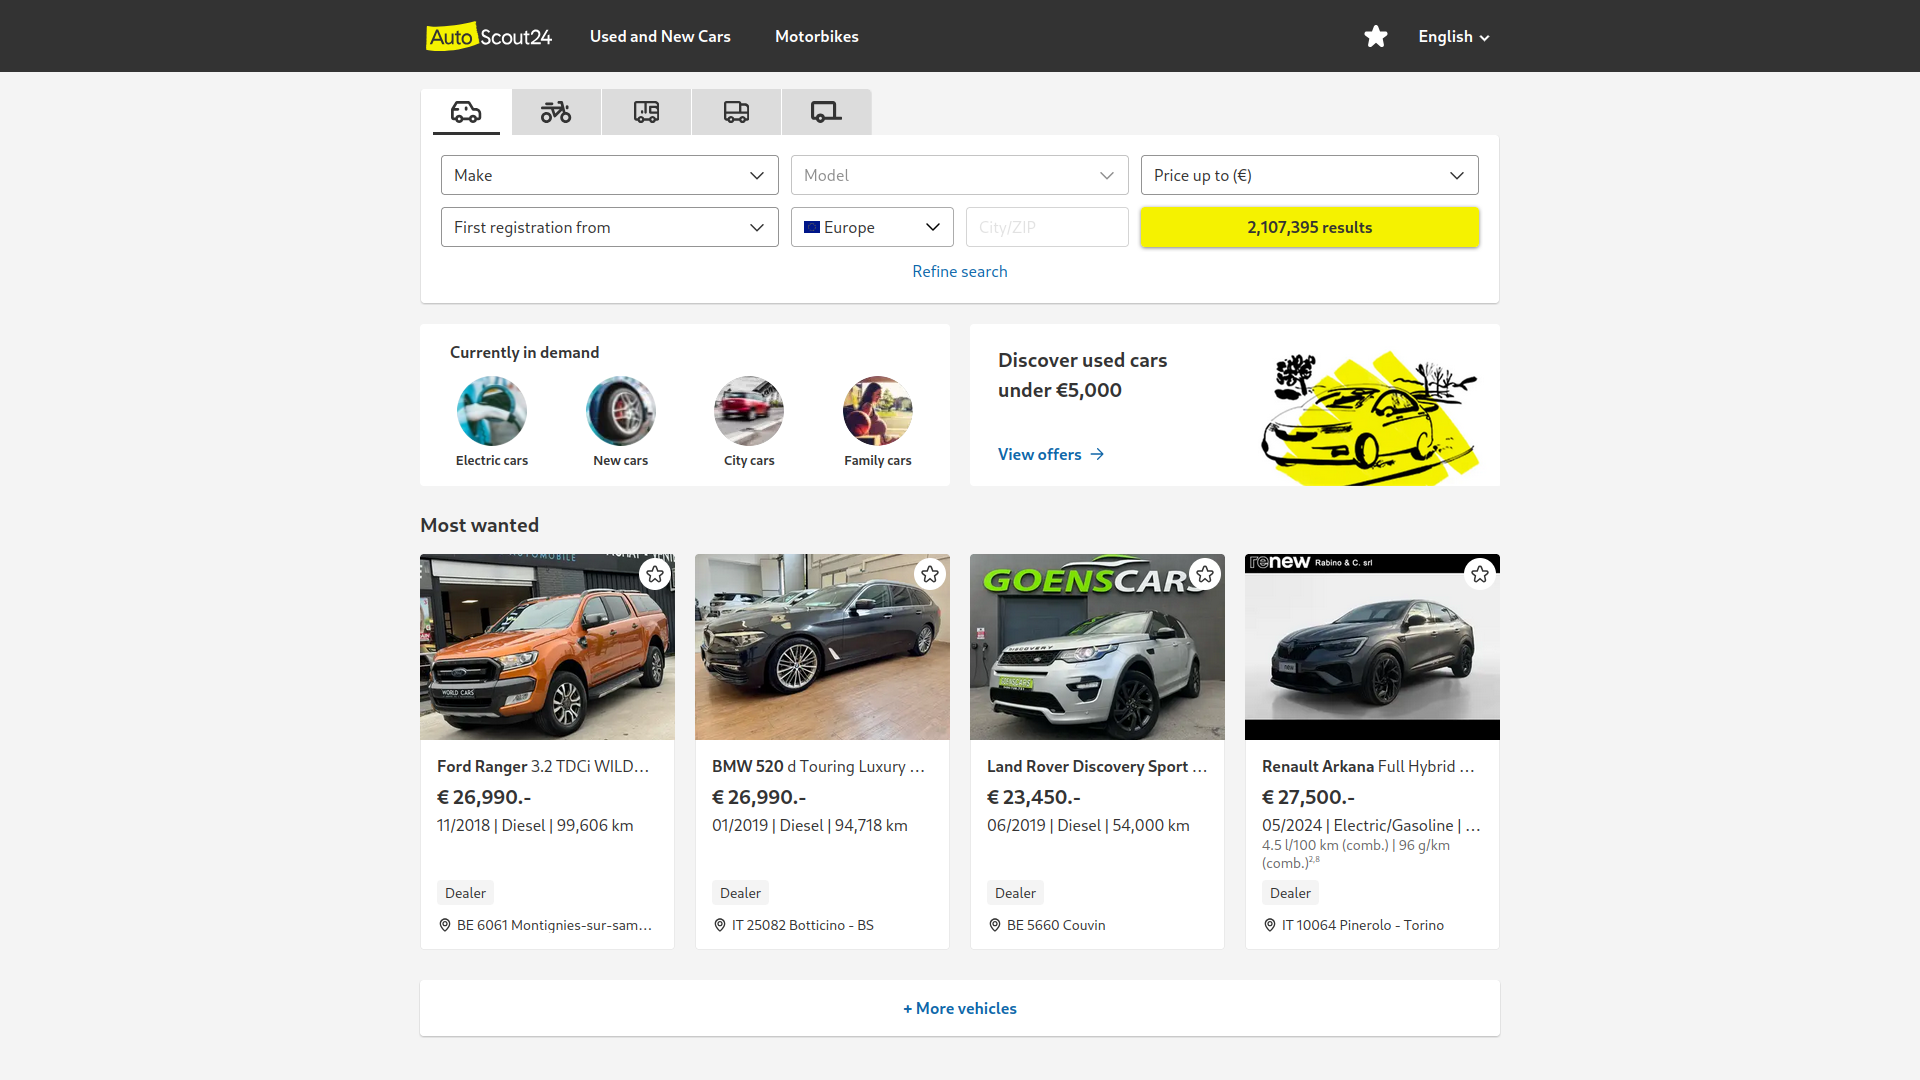
\includegraphics[width=\linewidth]{autoscout24.com}}
    \captionof{figure}{Скриншот главной страницы сайта autoscout24.com}
\end{minipage}
\bigskip

\noindent
\begin{minipage}{\linewidth}
    \fbox{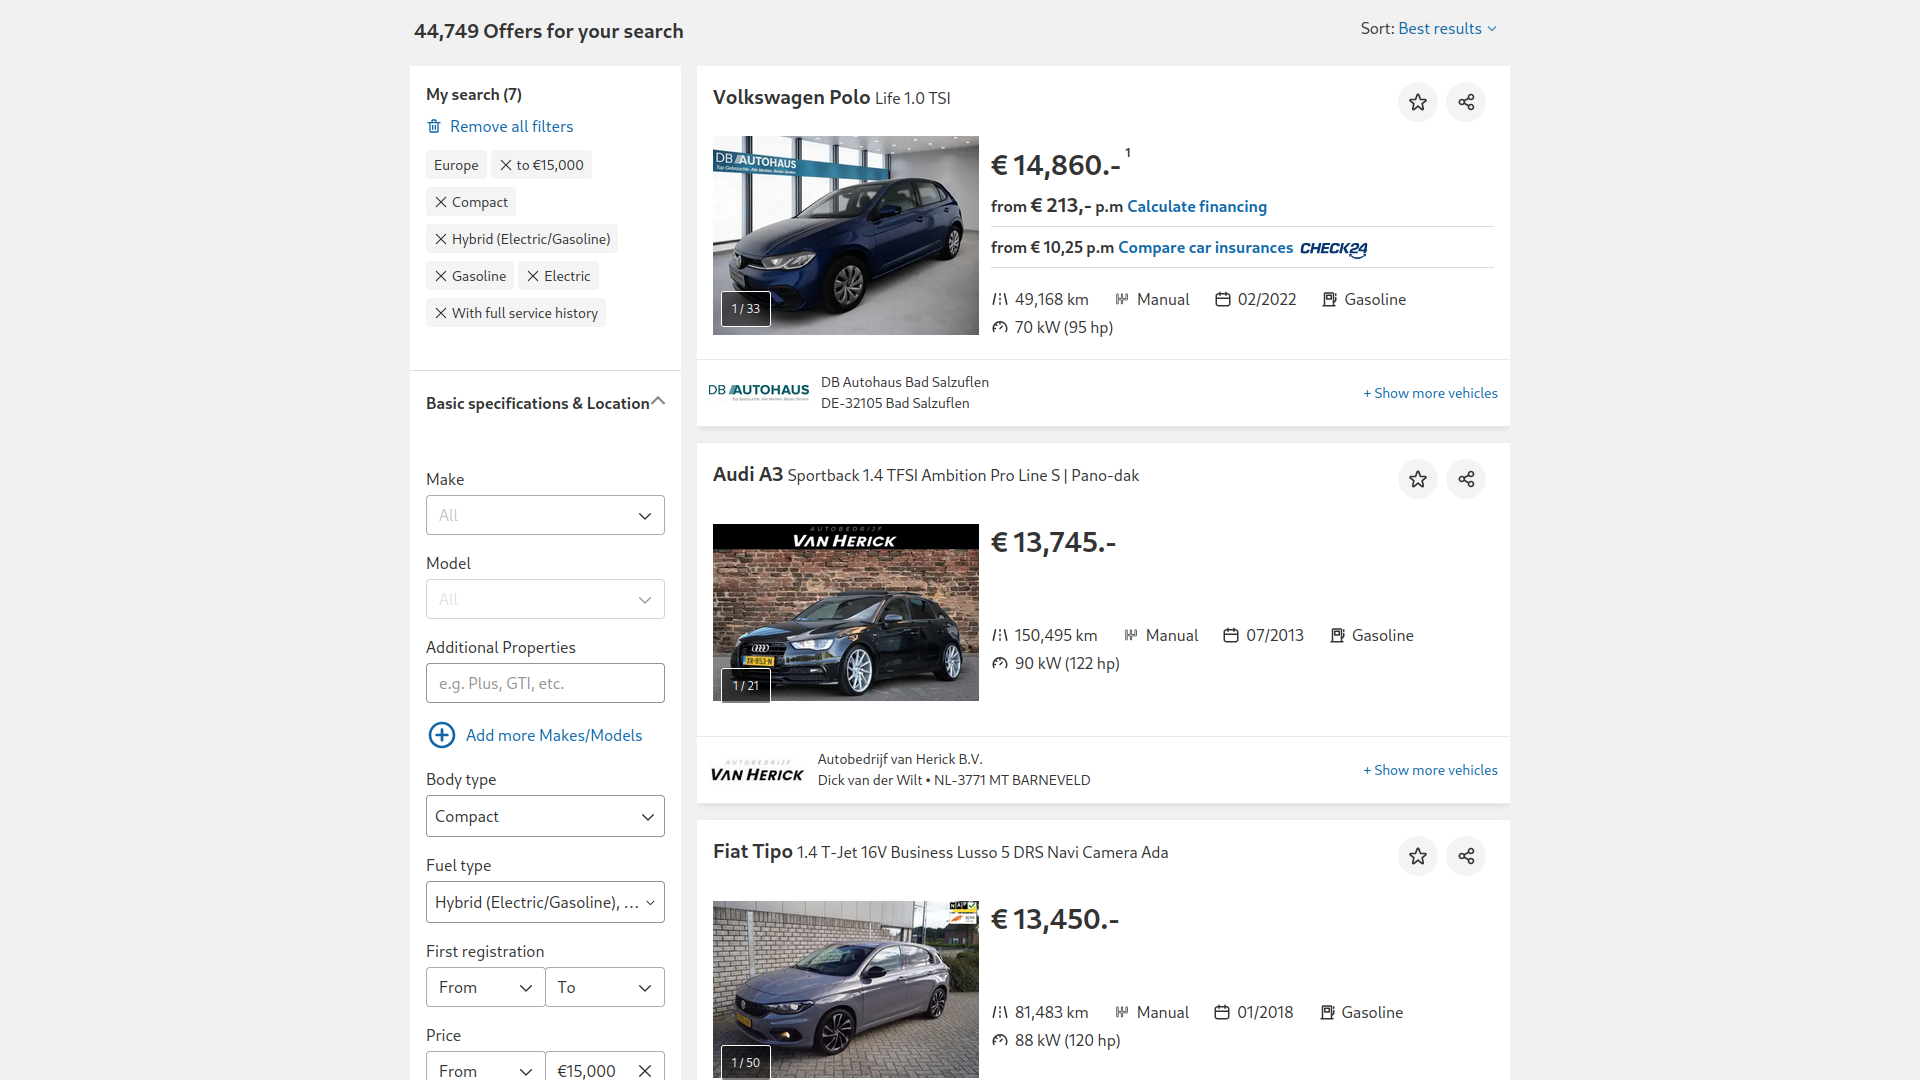
\includegraphics[width=\linewidth]{autoscout24.com2}}
    \captionof{figure}{Скриншот каталога автомобилей сайта autoscout24.com}
\end{minipage}
\bigskip

\noindent
\begin{minipage}{\linewidth}
    \fbox{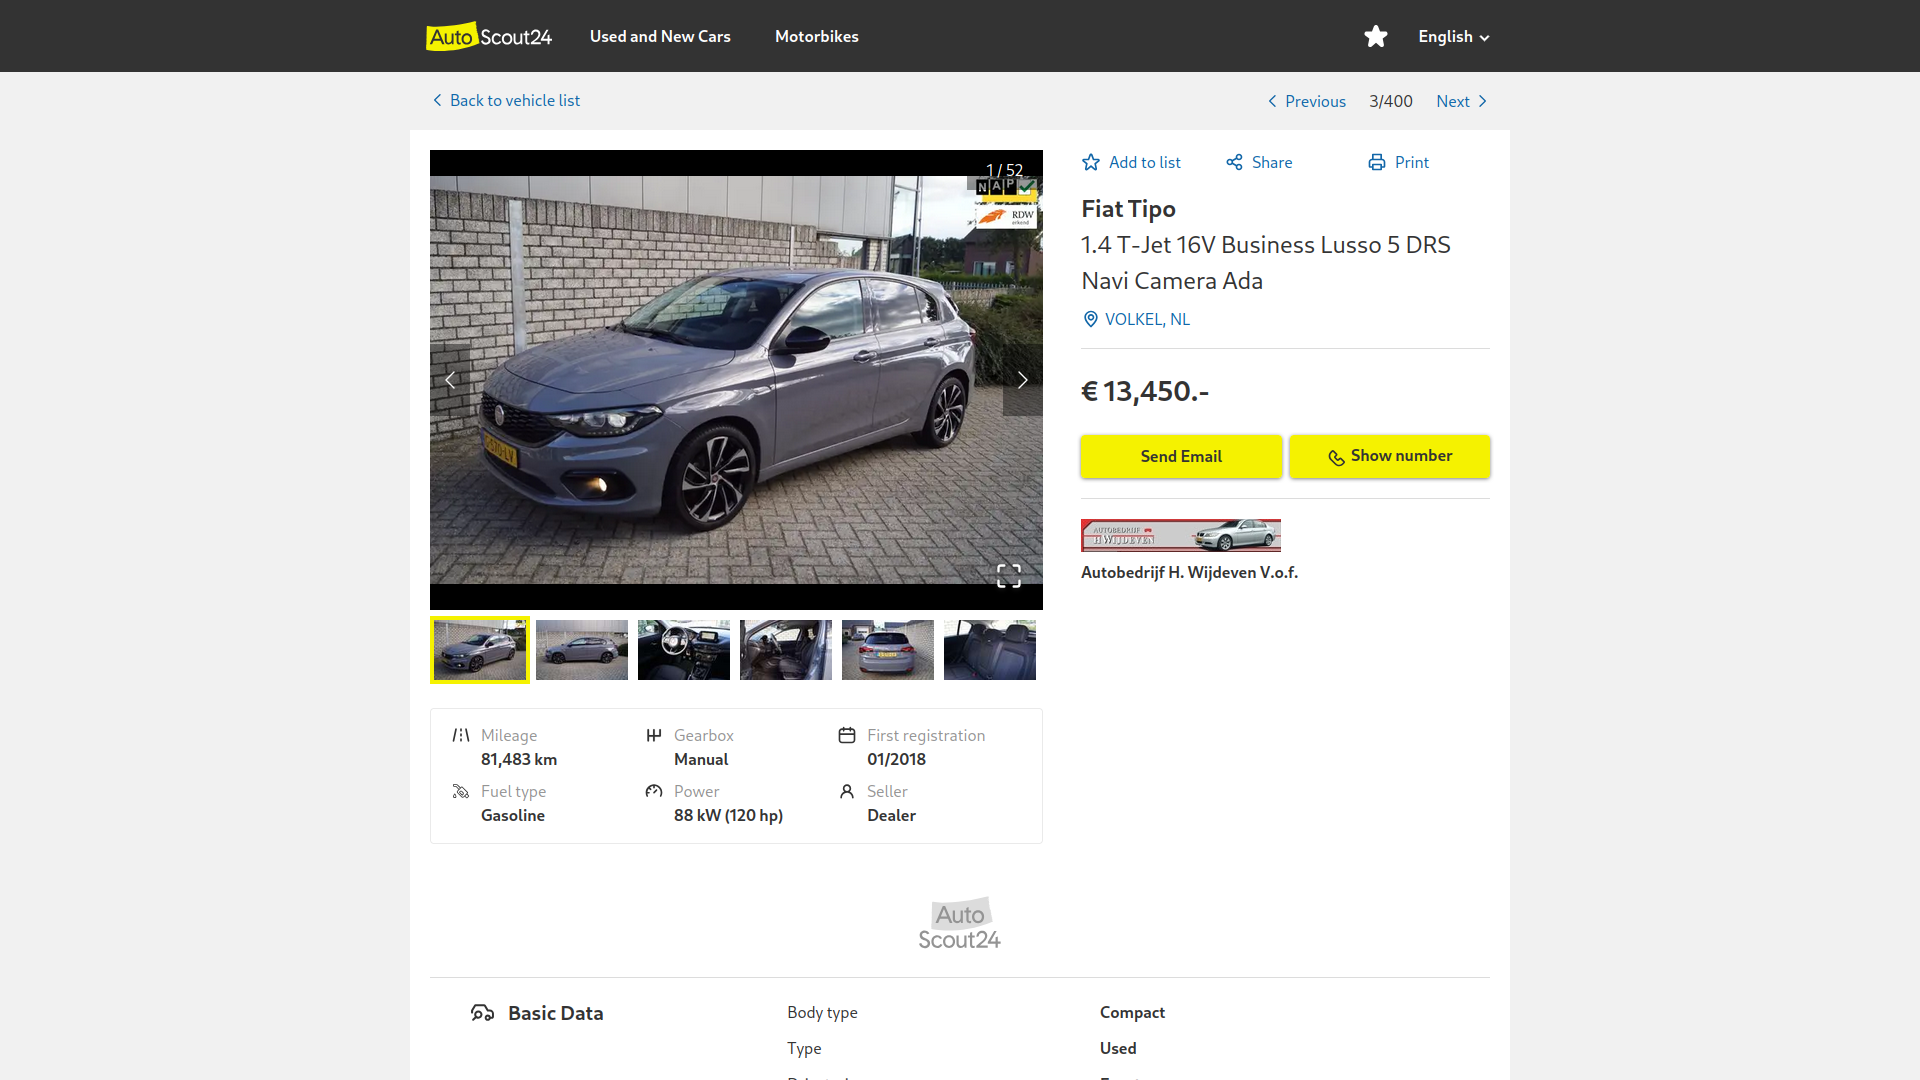
\includegraphics[width=\linewidth]{autoscout24.com3}}
    \captionof{figure}{Скриншот страницы выбора конкретного автомобиля сайта autoscout24.com}
\end{minipage}
\bigskip

Ниже представлены 2 таблицы, указывающие на популярность сайтов, а также на оценку таких их параметров, как: удобство, функциональность, и дизайн по пятибальной шкале.

\begin{table}[H]
    \centering
    \begin{tabular}{ | c | c | c | c | }
        \hline
        Сайт & Удобство & Функциональность & Дизайн\\
        \hline
        auto.ru & 4 & 5 & 4\\
        \hline
        drom.ru & 5 & 4 & 3\\
        \hline
        sberauto.com & 5 & 3 & 5\\
        \hline
        mobile.de & 4 & 4 & 5\\
        \hline
        autoscout24.com & 5 & 5 & 5\\
        \hline
    \end{tabular}
\end{table}

\begin{table}[H]
    \centering
    \small
    \begin{tblr}{
        cells = {c},
        cell{1}{1} = {r=2}{},
        cell{1}{2} = {c=2}{},
        cell{1}{4} = {r=2}{},
        cell{1}{5} = {r=2}{},
        cell{1}{6} = {r=2}{},
        cell{1}{7} = {r=2}{},
        vlines,
        hline{1,3-8} = {-}{},
        hline{2} = {2-3}{},
    }
    Сайт    & Рейтинг    &           & Визиты & Время & Отказ & {Страниц\\за визит } \\
            & Глобальный & Категория &        &       &       &                      \\
    auto.ru & 828 & 4 & 36.44M & 04:57 & 21.26\% & 9.90\\
    drom.ru & 317 & 1 & 75.61M & 08:03 & 36.93\% & 12.55\\
    sberauto.com & 112 748 & 1 185 & 266 886 & 10:45 & 26.12\% & 8.88\\
    mobile.de & 579 & 2 & 51.52M & 09:21 & 25.54\% & 9.98\\
    autoscout24.com & 13 182 & 114 & 3.853M & 03:53 & 31.76\% & 5.35
    \end{tblr}
\end{table}
\bigskip

\textbf{Бриф}
\bigskip

\begin{enumerate}
    \item Кто является вашей целевой аудиторией?\\
        Частные продавцы автомобилей, покупатели автомобилей, автосалоны и дилеры, автомобильные энтузиасты.
    \item Какие потребности и интересы у вашей целевой аудитории?\\
        Удобный поиск автомобилей, возможность быстро разместить объявление, получение информации о ценах и характеристиках, отзывы о продавцах.
    \item Какие функции вы хотите включить в сайт?\\
        Регистрация и авторизация пользователей, размещение объявлений, поиск и фильтрация по различным параметрам, сравнение автомобилей, система отзывов и рейтингов, интеграция с картами, мобильная версия.
    \item Какой стиль дизайна вы предпочитаете?\\
        Flat.
    \item Какие элементы навигации должны быть на сайте?\\
        Простая и интуитивно понятная навигация, меню с основными категориями и фильтрами.
    \item Есть ли у вас идеи для партнёрских программ с автосалонами?\\
        Да, сотрудничество с автосалонами и дилерами для увеличения базы объявлений.
    \item Какие конкуренты вы рассматриваете?\\
        auto.ru, drom.ru, sberauto.com, mobile.de, autoscout24.com.
    \item Какие сильные и слабые стороны у этих конкурентов?\\
        Сильные стороны конкурентов — широкий выбор автомобилей и развитая база пользователей. Слабые стороны — недостатки в удобстве/функциональности/дизайне.
    \item Каков ваш бюджет на разработку и продвижение сайта?\\
        Около 500,000 - 1,000,000 рублей на разработку и начальное продвижение.
    \item Какие сроки вы планируете для реализации проекта?\\
        3-6 месяцев.
    \item Какие типы транспортных средств будут представлены на сайте?\\
         На сайте будут представлены легковые автомобили, внедорожники, грузовики, мотоциклы и электромобили.
    \item Будет ли версия для слабовидящих людей и дальтоников?\\
        Нет
    \item Есть ли у вас идеи для интеграции с другими сервисами?\\
        Да, возможность интеграции с сервисами кредитования и страхования.
    \item Нужна ли поддержка нескольких языков на сайте?\\
        Да, это поможет привлечь более широкую аудиторию.
\end{enumerate}
\bigskip

\textbf{Вопросы к потенциальным пользователям сайта}
\bigskip

\begin{enumerate}
    \item Как часто вы покупаете или продаете автомобили?\\
        Я покупаю или продаю автомобили примерно раз в 2-3 года, в зависимости от необходимости.
    \item Какие факторы наиболее важны для вас при выборе платформы для размещения объявлений о продаже автомобилей?\\
        Важны удобство использования, наличие фильтров для поиска, безопасность сделок и возможность оставлять отзывы.
    \item Какие сайты вы уже использовали для покупки или продажи автомобилей? Почему именно их?\\
        Я использовал auto.ru и drom.ru, потому что они имеют большой выбор автомобилей и удобный интерфейс.
    \item Как вы оцениваете свой опыт использования текущих платформ для размещения объявлений? Что вам нравится, а что нет?\\
        В целом, опыт положительный. Нравится наличие большого количества объявлений, но иногда сложно найти нужный автомобиль из-за недостаточной фильтрации.
    \item Какие функции вы считаете наиболее полезными на сайтах по продаже автомобилей?\\
        Полезны фильтры по цене, пробегу и году выпуска, а также возможность сравнения автомобилей.
    \item С какими трудностями вы сталкивались при использовании существующих платформ?\\
        Иногда возникают проблемы с загрузкой фотографий и медленной работой сайта.
    \item Какие параметры вы обычно используете для поиска автомобилей (например, марка, модель, год выпуска, цена)?\\
        Я обычно ищу по марке, модели, году выпуска и цене.
    \item Насколько важна для вас возможность фильтрации и сортировки объявлений?\\
        Это очень важно, так как помогает быстро находить подходящие варианты.
    \item Как вы относитесь к возможности оставлять отзывы и оценки продавцам? Насколько это важно для вас?\\
        Это важно, так как отзывы помогают понять, насколько надежен продавец.
    \item Какую информацию вы хотели бы видеть в своем личном кабинете?\\
        Я хотел бы видеть свои объявления, историю покупок и продаж, а также уведомления о новых сообщениях.
    \item Какие функции вы хотели бы иметь в своем личном кабинете (например, управление объявлениями, история покупок/продаж, уведомления)?\\
        Управление объявлениями и уведомления о статусе сделок.
    \item Готовы ли вы платить за дополнительные услуги (например, выделение объявления)? Если да, то какие услуги вы считаете наиболее ценными?\\
        Да, я готов платить за выделение объявления и размещение на главной странице, если это увеличит шансы на продажу.
    \item Как вы относитесь к рекламе на сайте? Она вас отвлекает или вы считаете ее полезной?\\
        Реклама может быть полезной, если она релевантна, но слишком много рекламы отвлекает.
    \item На каких устройствах вы обычно используете сайты по продаже автомобилей (ПК, планшет, смартфон)?\\
        Я чаще всего использую смартфон, но иногда захожу с ПК.
    \item Насколько важно для вас, чтобы сайт был доступен на нескольких языках?\\
        Это не критично, но было бы удобно, если бы сайт поддерживал несколько языков.
\end{enumerate}
\bigskip

\textbf{Требования к разработке интерфейса сайта}
\bigskip

\begin{enumerate}
    \item Пользовательские требования
        \begin{itemize}
            \item Удобство использования: интерфейс должен быть интуитивно понятным и простым в навигации для пользователей с разным уровнем технической подготовки;
            \item Адаптивность: сайт должен корректно отображаться на различных устройствах (ПК, планшеты, смартфоны) и в разных браузерах;
            \item Регистрация и авторизация: пользователи должны иметь возможность легко зарегистрироваться и войти в систему с помощью электронной почты, социальных сетей или мобильного телефона;
            \item Личный кабинет: пользователи должны иметь доступ к личному кабинету, где они могут управлять своими объявлениями, просматривать историю действий и получать уведомления;
            \item Поиск и фильтрация: необходимо реализовать мощный функционал поиска и фильтрации объявлений по различным параметрам (марка, модель, год выпуска, цена, пробег и т.д.);
            \item Сортировка: необходимо реализовать функционал сортировки объявлений по различным параметрам (цена, год выпуска, популярность);
        \end{itemize}
    \item Функциональные требования
        \begin{itemize}
            \item создание объявления - пользователи должны иметь возможность создавать объявления с загрузкой фотографий, описанием, характеристиками автомобиля и ценой;
            \item редактирование и удаление объявлений - пользователи должны иметь возможность редактировать или удалять свои объявления в любое время;
            \item система уведомлений - пользователи должны получать уведомления о новых сообщениях, изменениях статуса объявлений и других важных событиях;
            \item интеграция с картами - возможность указания местоположения автомобиля на карте для удобства покупателей;
            \item система фильтров - фильтры для поиска автомобилей по различным критериям (например, по цене, году выпуска, пробегу и т.д.);
            \item сравнение автомобилей - возможность сравнения нескольких автомобилей по ключевым характеристикам;
        \end{itemize}
    \item Бизнес-требования
        \begin{itemize}
            \item внедрение платных услуг для продавцов (например, выделение объявления, размещение на главной странице);
            \item реклама на сайте (баннеры, контекстная реклама);
            \item поддержка нескольких языков - сайт должен поддерживать несколько языков для привлечения широкой аудитории.
        \end{itemize}
\end{enumerate}

\textbf{Контрольные вопросы и ответы}

\begin{enumerate}
    \item Основные типы сайтов и их характеристики.
        \begin{itemize}
            \item Информационные сайты - предназначены для предоставления информации о компании, продуктах, услугах или тематической области. Основная цель - информирование посетителей.
            \item Электронные коммерческие площадки - позволяют проводить торговые операции и совершать покупки и продажи товаров и услуг.
            \item Блоги и порталы - содержат периодически обновляемый контент на различные темы.
            \item Социальные сети - предназначены для социального взаимодействия и обмена информацией между пользователями.
        \end{itemize}
    \item Что такое эвристический анализ? Методика проведения эвристического анализа.

        Эвристический анализ - это метод оценки удобства использования интерфейса, основанный на принципах эвристического проектирования.

        Методика проведения:
        \begin{itemize}
            \item выбор эвристик - определение набора эвристик (эмпирических правил) оценки качества интерфейса;
            \item оценка интерфейса - эксперты оценивают интерфейс на соответствие выбранным эвристикам;
            \item выявление проблем - выявление ошибок и недостатков, которые нарушают выбранные эвристики;
            \item формирование рекомендаций - Формулирование рекомендаций по устранению выявленных проблем.
        \end{itemize}
    \item Что такое «бриф». Какие вопросы он должен содержать?

        Бриф - это документ, содержащий основные требования и пожелания заказчика к проекту.

        Основные вопросы:
        \begin{itemize}
            \item Цели и задачи проекта.
            \item Целевая аудитория.
            \item Требования к функционалу и дизайну.
            \item Бюджет и сроки реализации.
            \item Ожидаемые результаты и критерии успеха.
        \end{itemize}
    \item Как правильно сформулировать цель и задачи проектирования интерфейса информационной системы?

        Для достижения цели необходимо выполнить задачи. Чтобы правильно сформулировать задачи нужно придерживаться общей концепции:
изучение потребностей пользователей, разработка информационной архитектуры, проектирование пользовательского интерфейса. А для правильной формулировки цели нужно проанализировать потребности пользователя и выявить какую проблему решает интерфейс ИС.
    \item Каким требованиям должен отвечать проектируемый интерфейс?
        \begin{itemize}
            \item Удобство использования: интерфейс должен быть интуитивно понятным и легким в освоении для пользователей разного уровня опыта.
            \item Эффективность: пользователь должен легко достигать своих целей при работе с системой без излишних усилий и временных затрат.
            \item Надежность: интерфейс должен быть стабильным и безопасным для пользовательских данных.
            \item Привлекательный дизайн: дизайн должен быть привлекательным и соответствовать бренду или стилю компании.
            \item Адаптивность: интерфейс должен корректно отображаться на различных устройствах и в разных браузерах.
            \item Совместимость: интерфейс должен быть совместим с различными операционными системами и устройствами.
        \end{itemize}
\end{enumerate}

\end{document}
